\documentclass[a4paper, 11pt]{article}
\usepackage[margin=1in]{geometry}
\usepackage{preamble}

\title{ELEC4620 Assignment 1}
\author{Deren Teo}

\begin{document}

\maketitle

\section*{Question 1}
\fakesection{1}

The function for a rectangular pulse around $t=0$, with amplitude $A$ and width
$T$, is:
\begin{align*}
    h(t) = \begin{cases}
        A, & |t| < T/2 \\
        0, & |t| > T/2
    \end{cases}
\end{align*}
This is equivalent to two step functions of equal magnitude and opposite sign at
$t=\pm T/2$. Hence, the derivative of the rectangular pulse is composed of two
impulses of equal magnitude and opposite sign, coinciding in time with the
discontinuities in the pulse.
\begin{align*}
    h'(t) = A \delta(t+\frac{T}{2}) - A \delta(t-\frac{T}{2})
\end{align*}
Figure \ref{fig:q1_rectangular} visualises the rectangular pulse and its first
derivative.

\begin{figure}[ht]
    \centering
    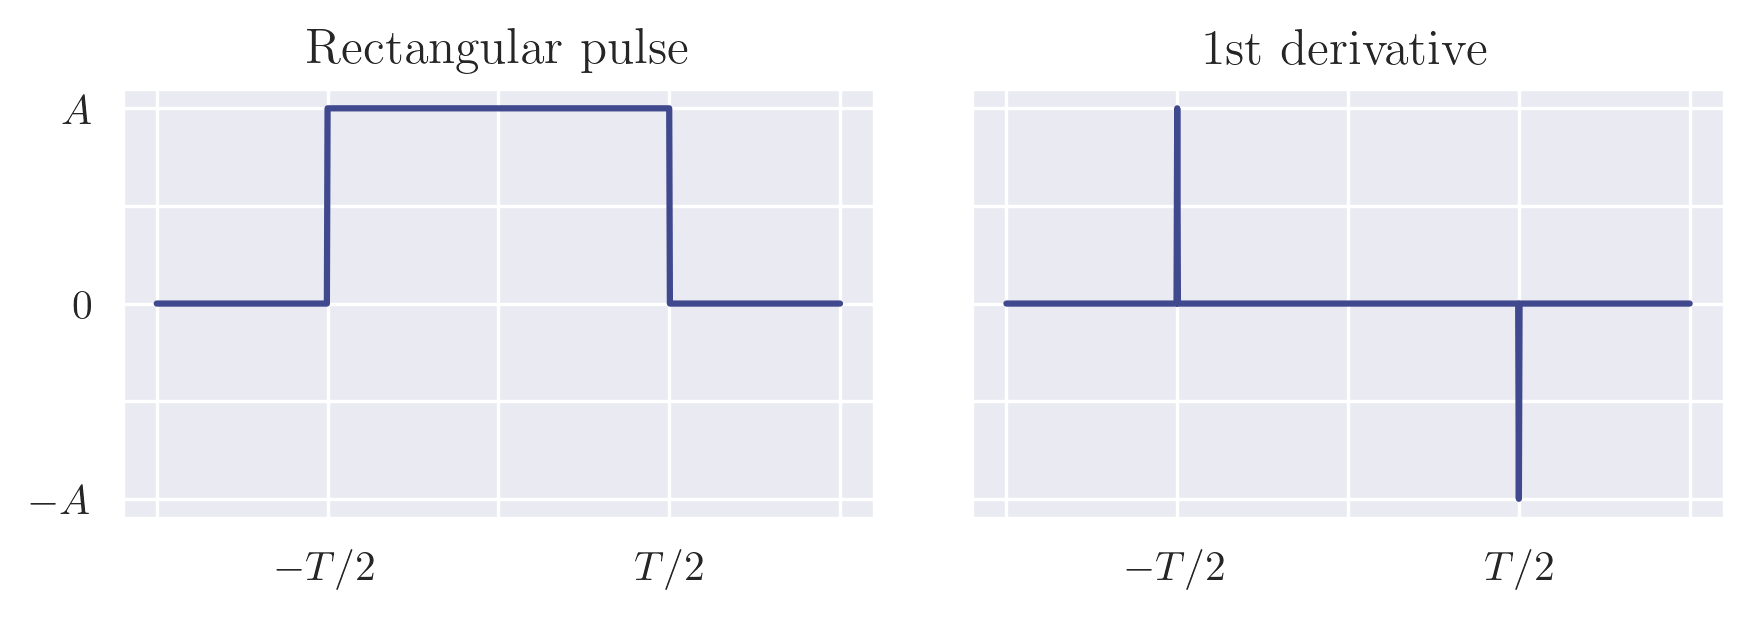
\includegraphics[width=0.66\textwidth]{images/q1_rectangular.png}
    \caption{A rectangular pulse and its first derivative}
    \label{fig:q1_rectangular}
\end{figure}

Writing out the Fourier transform of the derivative, which by definition is
\begin{align*}
    \widehat{H'}(f) \coloneqq \int_{-\infty}^{\infty} h'(t) e^{-j2\pi ft} dt
\end{align*}
we get the following expression, which has been split into two integrals for
simplicity.
\begin{align*}
    \widehat{H'}(f) = A \int_{-\infty}^{\infty} \delta(t + \frac{T}{2}) e^{-j2\pi ft} dt -
            A \int_{-\infty}^{\infty} \delta(t - \frac{T}{2}) e^{-j2\pi ft} dt
\end{align*}
By definition of the Dirac delta, $\delta(t-T)$, for arbitrary $T$:
\begin{align*}
    \delta(t-T) = \begin{cases}
        \infty, & t = T \\
        0,      & t \neq T
    \end{cases}
    && \text{and} &&
    \int_{-\infty}^{\infty} \delta(t-T) dt = 1
\end{align*}
Therefore, the Fourier transform of the derivative simplifies to
\begin{align*}
    \widehat{H'}(f) = Ae^{-j2\pi f(-T/2)} - Ae^{-j2\pi f(T/2)}
          = A \left[ e^{j\pi fT} - e^{-j\pi fT}\right]
\end{align*}
Finally, we can integrate in the time domain by dividing by $j2\pi f$ in the
frequency domain.
\begin{align*}
    H(f) = \frac{A}{j2\pi f} \left[ e^{j\pi fT} - e^{-j\pi fT}\right]
\end{align*}
Some re-arranging and substitutions can be performed to neaten the result, if desired:
\begin{align*}
    H(f) = \frac{A}{\pi f}\sin(\pi Tf)
         = AT\frac{\sin(\pi Tf)}{\pi Tf}
         = AT\text{sinc}(Tf)
\end{align*}
Thus, we have derived the Fourier transform of a rectangular pulse.

We now repeat this procedure for a triangle function using a double derivative.
The function for a triangular pulse around $t=0$, with amplitude $A$ and width $T$, is:
\begin{align*}
    h(t) = \begin{cases}
        A(1 - 2|t|/T), & |t| \leq T/2 \\
        0,             & |t| > T/2
    \end{cases}
\end{align*}
The first derivative produces a result composed of two rectangular pulses of
equal magnitude and opposite sign, or equivalently three step functions.
\begin{align*}
    h'(t) = \begin{cases}
        2A/T, & -T/2 \leq t \leq 0 \\
       -2A/T, &  0 \leq t \leq T/2 \\
        0,    & |t| > T/2
    \end{cases}
\end{align*}
Hence, as before, the second derivative is composed of three impulses coinciding
with the discontinuities in the first derivative.
\begin{align*}
    h''(t) = \frac{2A}{T}\delta(t+\frac{T}{2}) -
             \frac{4A}{T}\delta(t) +
             \frac{2A}{T}\delta(t-\frac{T}{2})
\end{align*}
Figure \ref{fig:q1_triangular} visualises the triangular pulse and its first and
second derivatives.

\begin{figure}[ht]
    \centering
    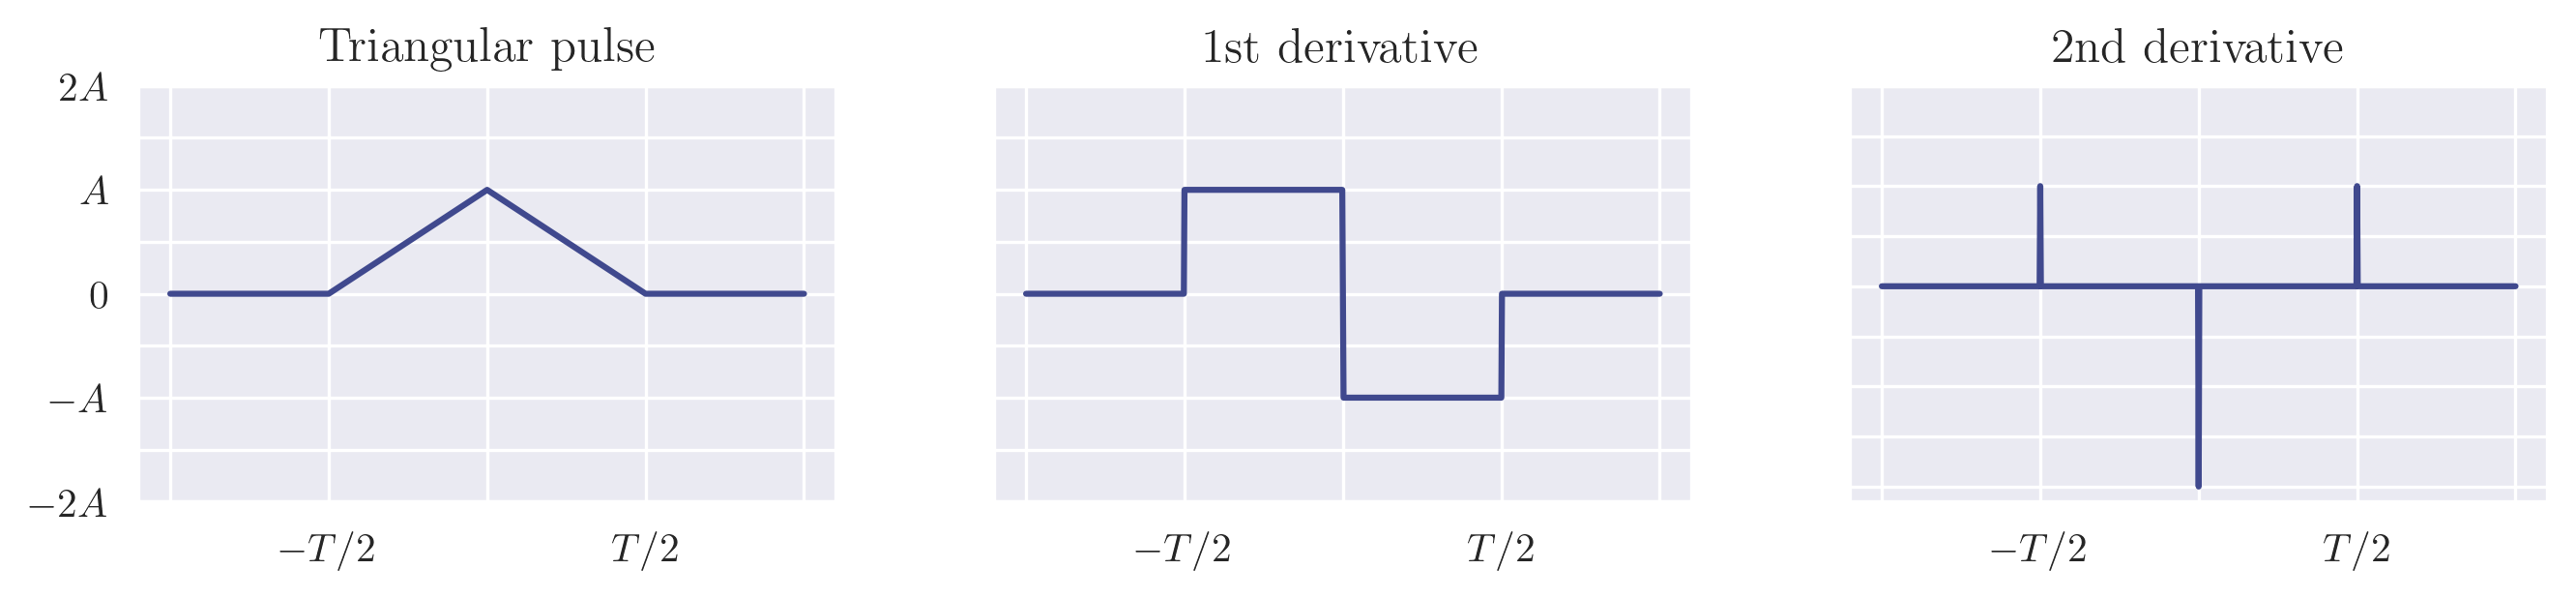
\includegraphics[width=0.99\textwidth]{images/q1_triangular.png}
    \caption{A triangular pulse and its first and second derivatives}
    \label{fig:q1_triangular}
\end{figure}

The Fourier transform of the second derivative is therefore
\begin{align*}
    \widehat{H''}(f) = \frac{2A}{T}\int_{-\infty}^\infty \delta(t+\frac{T}{2}) e^{-j2\pi ft} dt -
             \frac{4A}{T}\int_{-\infty}^\infty \delta(t) e^{-j2\pi ft} dt +
             \frac{2A}{T}\int_{-\infty}^\infty \delta(t-\frac{T}{2}) e^{-j2\pi ft} dt
\end{align*}
Once again, using the definition of the Dirac delta, the Fourier transform
simplifies to
\begin{align*}
    \widehat{H''}(f) = \frac{2A}{T} \left[ e^{-j2\pi f(-T/2)} - 2e^{-j2\pi f(0)} + e^{-j2\pi f(T/2)} \right]
\end{align*}
and further to
\begin{align*}
    \widehat{H''}(f) = \frac{2A}{T} \left[ e^{j\pi fT} - 2 + e^{-j\pi fT} \right]
\end{align*}
We can integrate twice in the time domain by dividing by $(j2\pi f)^2$ in the frequency
domain.
\begin{align*}
    H(f) = \frac{2A}{(j2\pi f)^2 T} \left[ e^{j\pi fT} - 2 + e^{-j\pi fT} \right]
         = \frac{-A}{2\pi^2f^2 T} \left[ e^{j\pi fT} - 2 + e^{-j\pi fT} \right]
\end{align*}
Finally, as with the rectangular pulse, we can re-arrange this result into a
more familiar form:
\begin{align*}
    H(f) = \frac{A}{\pi^2f^2T}(1 - \cos(\pi Tf))
         = \frac{AT}{2} \text{sinc}^2(\frac{Tf}{2})
\end{align*}
Thus, we have derived the Fourier transform of a triangular pulse.

Having derived the Fourier transforms of the two functions, we are interested in
comparing the rates at which their magnitudes decrease as frequency increases.
We note the only term contributing to a change in magnitude with frequency is
the $1/f$ term for the rectangular pulse, and the $1/f^2$ term for the
triangular pulse.

Indeed, in general, if a function has discontinuities in the $n^\text{th}$
derivative, the sidelobes of its Fourier transform will fall off as $1/f^{n+1}$.
Intuitively, this is because the function must be derived $n+1$ times to obtain
a number of impulses which can be Fourier transformed without yielding any
frequency-dependent coefficients. The transform of the derivative is then
integrated $n+1$ times by dividing by $(j2\pi f)^{n+1}$; hence, the term
$1/f^{n+1}$ is produced.

Figure \ref{fig:q1_sidelobes} presents the Fourier transforms of the rectangular
and triangular pulses, enabling a visual comparison of the rates at which their
sidelobes fall off.

\begin{figure}[ht]
    \centering
    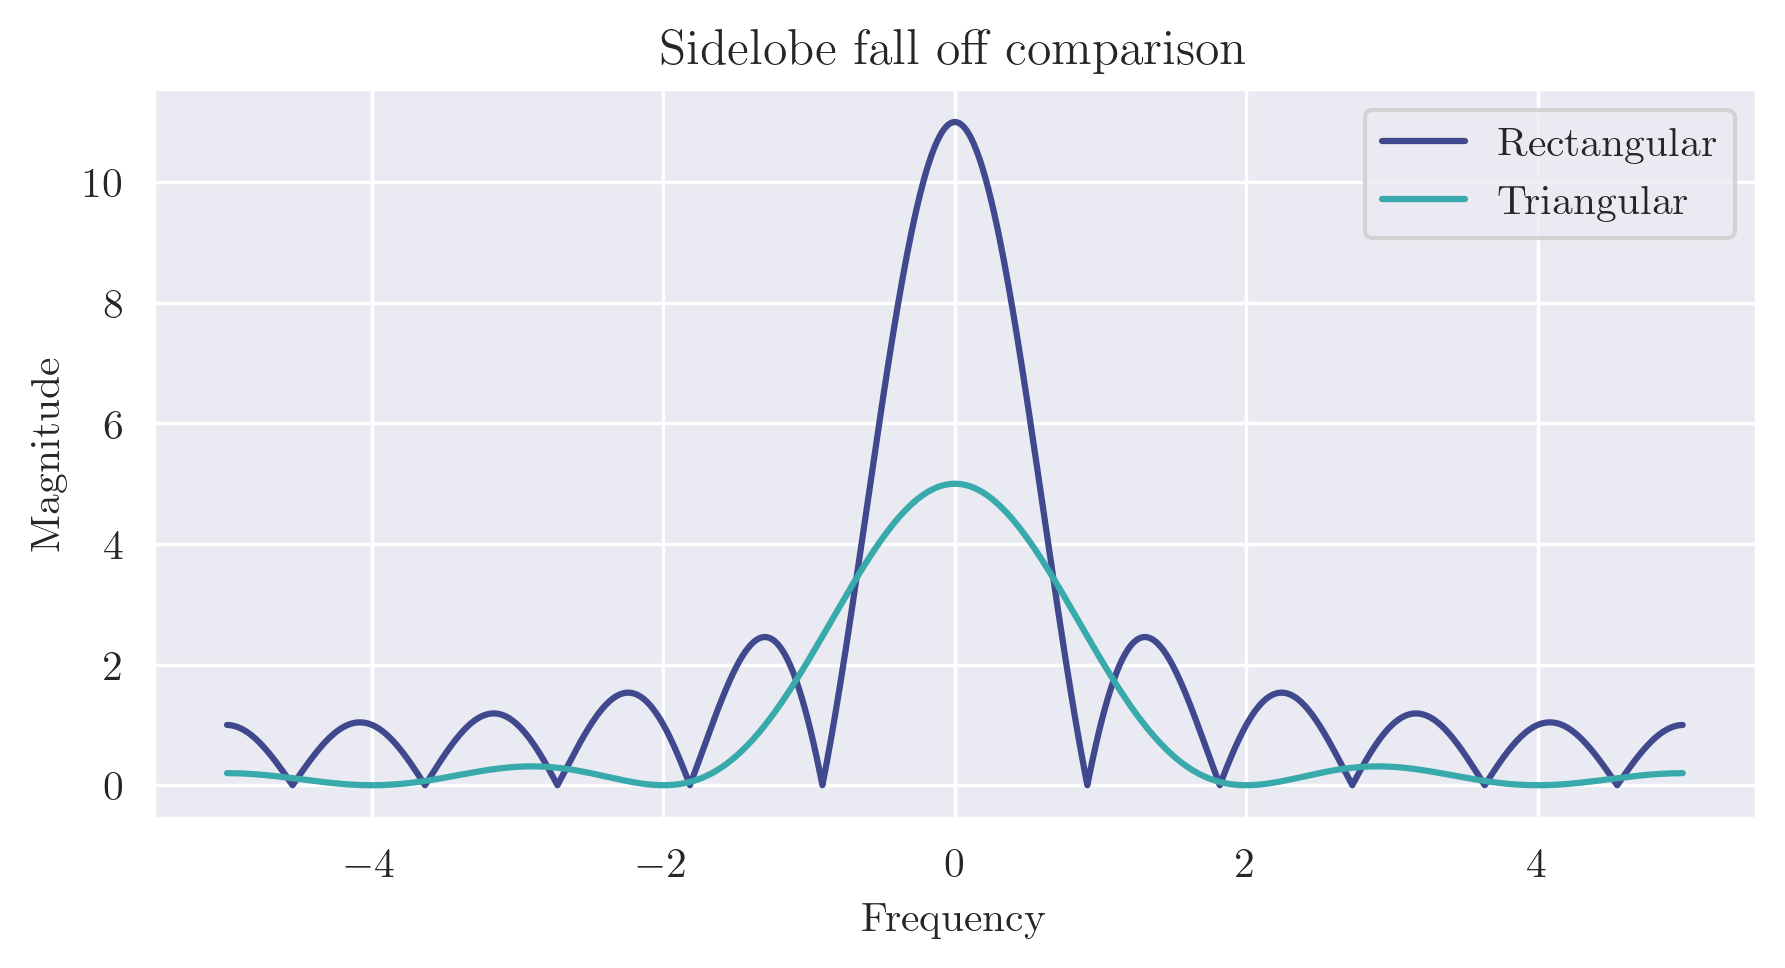
\includegraphics[width=0.95\textwidth]{images/q1_sidelobes.png}
    \caption{Fourier transform sidelobe fall off comparison: rectangular and
             triangular pulses.}
    \label{fig:q1_sidelobes}
\end{figure}

The full python code for this question, and all following questions, can be
found in the Appendix.

\newpage
\section*{Question 2}
\fakesection{2}

Denote the given polynomials in $z$ by $X(z)$ and $Y(z)$, as follows:
\begin{align*}
    X(z) &= 1 + 2z^{-1} + 6z^{-2} + 11z^{-3} + 15z^{-4} + 12z^{-5} \\
    Y(z) &= 1 - 3z^{-1} - 3z^{-2} + 7z^{-3} - 7z^{-4} + 3z^{-5}
\end{align*}
Their corresponding vectors are constructed from their respective coefficients:
\begin{align*}
    v_X = [1, 2, 6, 11, 15, 12] && \text{and} && v_Y = [1, -3, -3, 7, -7, 3]
\end{align*}
The result of multiplying $X(z)$ and $Y(z)$ can be obtained by convolving their
respective vectors and interpreting the outcome as the coefficients of the
polynomial product. That is,
\begin{align*}
    X(z)Y(z) = \sum_{i=0}^{M+N-1} (v_X \ast v_Y)_i z^{-i}
    % v_X \ast v_Y = [1, -1, -3, -6, -29, -35, -40, 10, 12, -39, 36]
\end{align*}
where $M$ and $N$ are the lengths of $v_X$ and $v_Y$, respectively, and
$(v_X\ast v_Y)_i$ denotes the $i^\text{th}$ element of the vector produced by
the convolution of $v_X$ with $v_Y$. In terms of the latter, $v_X\ast v_Y$ can
be calculated using the \texttt{convolve} function from the
\texttt{scipy.signal} library:
\begin{center}
    \texttt{signal.convolve(vx, vy, mode="full", method="direct")}
\end{center}
This calculates the full discrete linear convolution, automatically
zero-padding the vectors as necessary, using traditional convolution (i.e.
multiplying and summing, as opposed to the FFT). The result is:
\begin{align*}
    v_X \ast v_Y = [1, -1, -3, -6, -29, -35, -40, 10, 12, -39, 36]
\end{align*}
Hence, we can interpret the convolution result as the polynomial product of
$X(z)$ and $Y(z)$:
\begin{align*}
    1 - z^{-1} - 3z^{-2} - 6z^{-3} - 29z^{-4} - 35z^{-5} - 40z^{-6} + 10z^{-7} +
    12z^{-8} - 39z^{-9} + 36z^{-10}
\end{align*}
Since convolution is equivalent to multiplication in the Fourier domain, we
could equivalently Fourier transform both vectors, multiply in the Fourier
domain, then perform an inverse Fourier transform to obtain the same vector of
coefficients derived above.

To demonstrate this in Python, we manually zero-pad the vectors before
performing the FFT.
\begin{center}
    \texttt{v\_x = np.pad(v\_x, (0, len(v\_y) - 1))} \\
    \texttt{v\_y = np.pad(v\_y, (0, len(v\_x) - 1))}
\end{center}
Here, the \texttt{numpy} package is used to zero-pad both vectors to the right
to the appropriate length. Then, \texttt{fft} and \texttt{ifft} from
\texttt{scipy.fft} can be applied:
\begin{center}
    \texttt{ifft(fft(v\_x) * fft(v\_y))}
\end{center}
This calculates the following vector, which, as expected, is identical to the
vector determined through direct convolution:
\begin{center}
    \texttt{[  1.  -1.  -3.  -6. -29. -35. -40.  10.  12. -39.  36.]}
\end{center}
Hence, the coefficients of the product of two polynomials can be determined from
either convolving vectors of their respective coefficients, or by Fourier
transforming those vectors, multiplying them together, then taking the inverse
Fourier transform of the result.

\newpage
\section*{Question 3}
\fakesection{3}

Given the following numbers in base 10, we seek to apply similar methods to
Question 2 to multiply the numbers, first using convolution, then using Fourier
transform techniques.
\begin{align*}
    x = 8755790 && \text{and} && y = 1367267
\end{align*}
Before that, however, we can perform regular multiplication to determine the
correct answer:
\begin{align*}
    8755790 \times 1367267 = 11971502725930
\end{align*}
Having done that, we construct the numbers digit-wise into vectors:
\begin{align*}
    v_x = [8, 7, 5, 5, 7, 9, 0] && \text{and} && v_y = [1, 3, 6, 7, 2, 6, 7]
\end{align*}
As before, the result of multiplying $x$ and $y$ can be obtained by convolving
their respective vectors. However, the ``carry" step must then be performed to
produce a number in base 10. This will become clearer after the convolution has
been performed.

Using the same \texttt{signal.convolve} method from Question 2, the following
result is determined:
\begin{align*}
    v_x \ast v_y = [8, 31, 74, 118, 117, 157, 212, 192, 142, 95, 103, 63, 0]
\end{align*}
Now, however, unlike with polynomial multiplication, we cannot expect to
arrive at the correct product by simply stringing together all the digits.
Instead, starting from the right, each value must be taken modulo 10, and the
remainder added to the value immediately to the left. This yields the following
base-10 vector, which can now be concatenated into the product of $x \times y$:
\begin{align*}
    [1, 1, 9, 7, 1, 5, 0, 2, 7, 2, 5, 9, 3, 0] \longrightarrow 11971502725930
\end{align*}
Naturally, the same outcome can be achieved by Fourier transforming the vectors,
multiplying in the Fourier domain, then inverse Fourier transforming the result.
Again, in Python, the vectors must be zero-padded before performing the FFT.
\begin{center}
    \texttt{v\_x = np.pad(v\_x, (0, len(v\_y) - 1))} \\
    \texttt{v\_y = np.pad(v\_y, (0, len(v\_x) - 1))}
\end{center}
Then, in the same manner as Question 2:
\begin{center}
    \texttt{ifft(fft(v\_x) * fft(v\_y))} =
        [8.  31.  74. 118. 117. 157. 212. 192. 142.  95. 103.  63.   0.]
\end{center}
As expected, the vector produced by this method is identical to that produced by
direct convolution. Therefore, if we apply the same ``carrying'' process that we
applied above, we will no doubt arrive at the same value for the product of
$x\times y$.

Hence, integer multiplication also can be accomplished by either convolving the
vector representations of the numbers and converting to base 10, or multiplying
the Fourier transforms of the vectors, then taking the inverse Fourier transform
and converting to base 10.

\newpage
\section*{Question 4}
\fakesection{4}

\begin{enumerate}[label=\alph*)]

    \item First, we individually transform the sequences using the \texttt{fft}
    function from \texttt{scipy.fft}:
    \begin{align*}
        \texttt{fft(x)} = [&34,\ -1.879+j6.536,\ -5+j7,\ -6.121+j0.536,\ \\
                           &0,\ -6.121-j0.536,\ -5-j7,\ -1.879-j6.536] \\
        \texttt{fft(y)} = [&28,\ 2.243+j4.243,\ -2-j2,\ -6.243+j4.243,\ \\
                           &-8,\ -6.243-j4.243,\ -2+j2,\ 2.243-j4.243]
    \end{align*}
    This gives us the expected result of the double transform algorithm. Now, to
    proceed, we combine $x$ and $y$ element-wise into a single complex vector:
    \begin{align*}
        z = [1+j,\ 2+j5,\ 4+j3,\ 4+j,\ 5+j3,\ 3+j5,\ 7+j3,\ 8+j7]
    \end{align*}
    We can use the same \texttt{fft} function without any additional
    considerations to Fourier transform this complex vector. Doing so, we
    obtain:
    \begin{align*}
        \texttt{fft(z)} = [&34+j28,\ -6.121+j8.778,\ -3+j5,\ -10.364-j5.707,\ \\
                           &-j8,\ -1.879-j6.778,\ -7-j9,\ 2.364-j4.293]
    \end{align*}
    The Fourier transforms of $x$ and $y$ can be determined from the
    Fourier transform of $z$ as
    \begin{align*}
        X &= \Ev(\Re(Z)) + j\Od(\Im(Z)) \\
        Y &= \Ev(\Im(Z)) - j\Od(\Re(Z))
    \end{align*}
    where $Z$ is the Fourier transform of $z$. Since $x$ is purely real and $y$
    purely imaginary, the Fourier transform of $x$ has a purely even real
    component and purely odd imaginary component, and vice versa for the Fourier
    transform of $y$. Even and odd components are orthogonal; hence, $X$ and $Y$
    can be independently reconstructed.

    The even and odd components of a sequence $H(n)$ are determined as:
    \begin{align*}
        \Ev(n) = \frac{H(n)+H(-n)}{2} && \Od(n) = \frac{H(n)-H(-n)}{2}
    \end{align*}
    where $H(-n)$ is the vector $H$ with all elements after the first in
    reversed order. Hence,
    \begin{align*}
        \Ev(\Re(Z)) &= [34,\ -1.879,\ -5,\ -6.121,\ 0,\ -6.121,\ -5,\ -1.879] \\
        \Od(\Im(Z)) &= [0,\ 6.536,\ 7,\ 0.536,\ 0,\ -0.536,\ -7,\ -6.535] \\
        \Ev(\Im(Z)) &= [28,\ 2.243,\ -2,\ -6.243,\ -8,\ -6.243,\ -2,\ 2.243] \\
        \Od(\Re(Z)) &= [0,\ -4,\ 243,\ 2,\ -4,243,\ 0,\ 4.243,\ -2,\ 4.243]
    \end{align*}
    wherein from the second element of each vector onward, the even and odd
    symmetries can be observed. Finally, we can reconstruct the individual
    Fourier transforms of $x$ and $y$:
    \begin{align*}
        X = [&34,\ -1.879+j6.536,\ -5+j7,\ -6.121+j0.536,\ \\
             &0,\ -6.121-j0.536,\ -5-j7,\ -1.879-j6.536] \\
        Y = [&28,\ 2.243+j4.243,\ -2-j2,\ -6.243+j4.243,\ \\
             &-8,\ -6.243-j4.243,\ -2+j2,\ 2.243-j4.243]
    \end{align*}
    Comparing these vectors to those determined individually at the start, we
    can see they are identical. Therefore, we have shown that the double
    transform algorithm gives the same answer as directly transforming the
    sequences.

\newpage

    \item In the previous part, the double transform algorithm was applied to
    sequences of equal length. However, it is also applicable to sequences of
    unequal length by right-padding the shorter sequence with zero. For example,
    \begin{align*}
        x = [1\ 2\ 4\ 4\ 5\ 3\ 7\ 8] &&
        y = [1\ 5\ 3\ 1\ 3\ 5\ 3\ \textcolor{red}{0}]
    \end{align*}
    The individual Fourier transforms of $x$ and $y$ are:
    \begin{align*}
        \texttt{fft(x)} = [&34,\ -1.879+j6.536,\ -5+j7,\ -6.121+j0.536 \\
                           &0,\ -6.121-j0.536,\ -5-j7,\ -1.879-j6.536] \\
        \texttt{fft(y)} = [&21,\ -2.707-j0.707,\ -2-j9,\ -1.293-j0.707 \\
                           &-1,\ -1.293+j0.707,\ -2+j9,\ -2.707+j0.707]
    \end{align*}
    As before, we combine $x$ and $y$ element-wise into a single complex vector:
    \begin{align*}
        z = [1+j\ \ 2+j5\ \ 4+j3\ \ 4+j\ \ 5+j3\ \ 3+j5\ \ 7+j3\ \ 8+j0]
    \end{align*}
    Using \texttt{scipy.fft}, the Fourier transform of $z$ is
    \begin{align*}
        \texttt{fft(z)} = [&34+j21,\ -1.172+j3.828,\ 4+j5,\ -5.414-j0.757,\\
                           &-j,\ -6.828-j1.828,\ -14-j9,\ -2.586-j9.243]
    \end{align*}
    Akin to part (a), the Fourier transforms of $x$ and $y$ can individually be
    determined from $Z$ using the even and odd components of the real and
    imaginary parts of $Z$.
    \begin{align*}
        \Ev(\Re(Z)) &= [34,\ -1.879,\ -5,\ -6.121,\ 0,\ -6.121,\ -5,\ -1.879] \\
        \Od(\Im(Z)) &= [0,\ 6.536,\ 7,\ 0.536,\ 0,\ -0.536,\ -7,\ -6.536] \\
        \Ev(\Im(Z)) &= [0,\ 0.707,\ 9,\ 0.707,\ 0,\ -0.707,\ -9,\ -0.707] \\
        \Od(\Re(Z)) &= [21,\ -2.707,\ -2,\ -1.293,\ -1,\ -1.293,\ -2,\ -2.707]
    \end{align*}
    Finally, we can reconstruct the individual Fourier transforms of $x$ and
    $y$:
    \begin{align*}
        X = [&34,\ -1.879+j6.536,\ -5+j7,\ -6.121+j0.536 \\
             &0,\ -6.121-j0.536,\ -5-j7,\ -1.879-j6.536] \\
        Y = [&21,\ -2.707-j0.707,\ -2-j9,\ -1.293-j0.707 \\
             &-1,\ -1.293+j0.707,\ -2+j9,\ -2.707+j0.707]
    \end{align*}
    Comparing these vectors to those determined individually at the start, we
    can see they are identical. We can additionally check that the shorter
    sequence can be recovered using the inverse Fourier transform:
    \begin{align*}
        \texttt{ifft(Y) = [ 1.  5.  3.  1.  3.  5.  3. -0.]}
    \end{align*}
    Given we know how many zeros were padded onto the shorter sequence, it can
    indeed be recovered by truncating the extra length. Therefore, the double
    transform algorithm can be applied even if the sequences differ in length.

\end{enumerate}

\newpage
\section*{Question 5}
\fakesection{5}

\begin{enumerate}[label=\alph*)]

    \item We are given the following polynomial, and want to determine its poles
    and zeros.
    \begin{align*}
        F(z) = 1 + 5z^{-1} + 3z^{-2} + 4z^{-3} + 4z^{-4} + 2z^{-5} + z^{-6}
    \end{align*}
    The absence of a denominator indicates an all-zero model (or, more
    accurately, all poles occur at the origin and are thus omitted from the
    pole-zero plot). In canonical form:
    \begin{align*}
        F(z) \cdot \frac{z^6}{z^6} = \frac{1 + 2z + 4z^{2} + 4z^{3} + 3z^{4} +
            5z^{5} + z^{6}}{z^6}
    \end{align*}
    The coordinates of the zeros are the complex roots of the numerator of
    $F(z)$, which can be found using \texttt{numpy.polynomial}:
    \begin{center}
        \texttt{Polynomial([1, 2, 4, 4, 3, 5, 1]).roots()}
    \end{center}
    This finds the following six roots:
    \begin{align*}
        z = -4.490,\ -0.751,\ -0.221\pm j0.551,\ 0.342\pm j0.852
    \end{align*}
    Figure \ref{fig:q5a_polezero} plots these on the complex plane, with the unit
    circle for reference.
    \begin{figure}[ht]
        \centering
        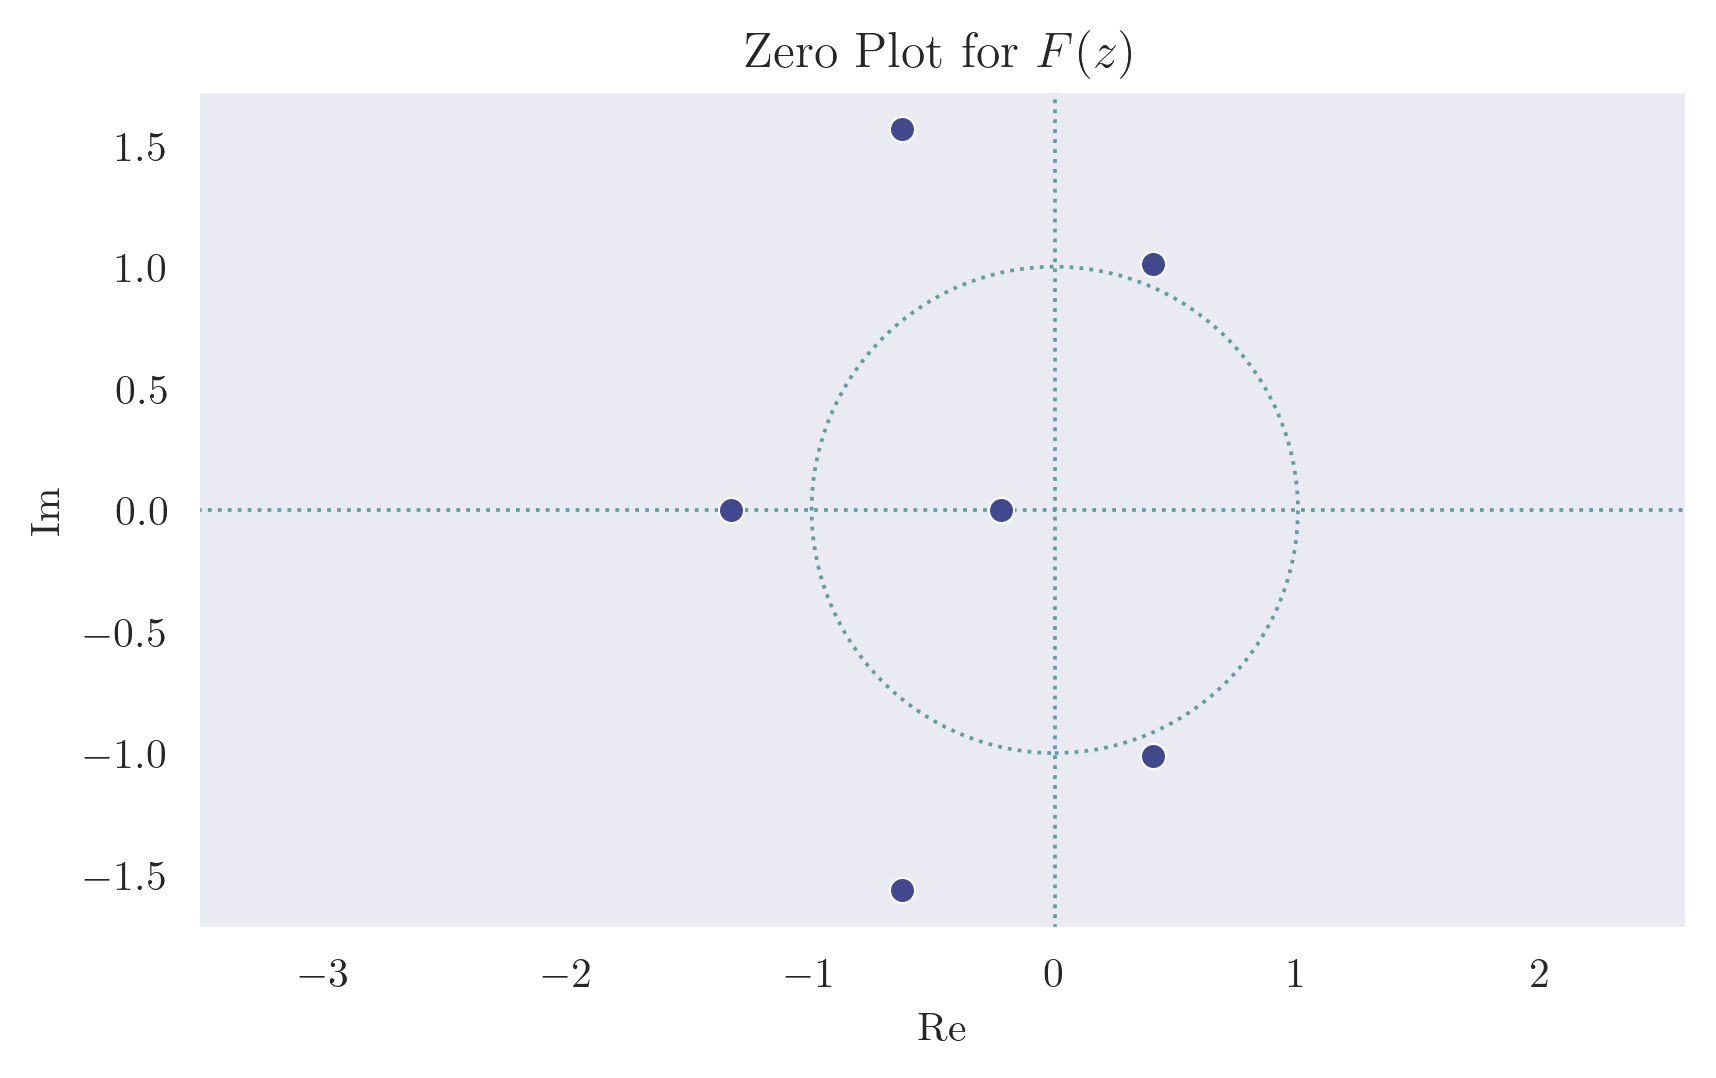
\includegraphics[width=0.8\textwidth]{images/q5a_polezero.png}
        \caption{Zero plot for $F(z)$; no poles are present.}
        \label{fig:q5a_polezero}
    \end{figure}

\newpage

    \item The sinusoidal steady-state response of the system can be modelled by
    evaluating the magnitude of $F(z)$ around the unit circle, which is
    effectively what is done by the DFT.

    That is,
    \begin{align*}
        F(z) \big|_{z=e^{-j2\pi k/N},\ k=0,\ldots,N-1}
    \end{align*}
    Figure \ref{fig:q5b_dftsample} compares \texttt{scipy.fft} and a
    self-implemented DFT function for $N=128$.
    \begin{figure}[ht]
        \centering
        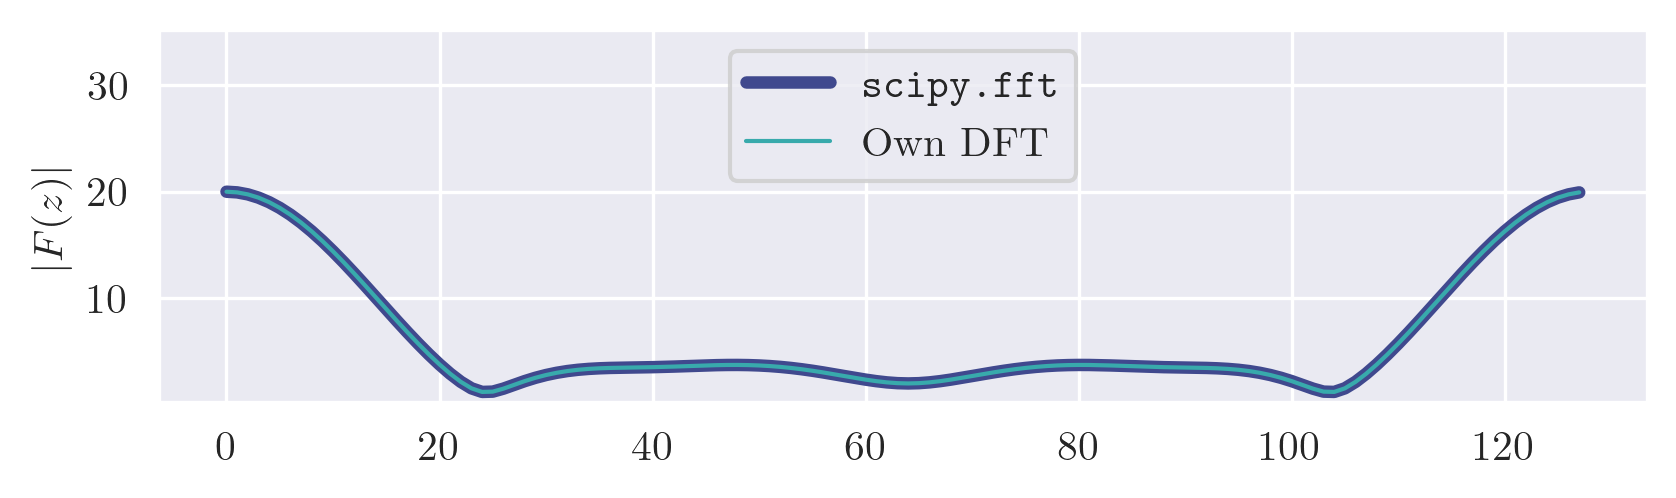
\includegraphics[width=0.8\textwidth]{images/q5b_dftsample.png}
        \caption{$|F(z)|$ evaluated at 128 points around the unit circle.}
        \label{fig:q5b_dftsample}
    \end{figure}

\end{enumerate}

\newpage
\section*{Question 6}
\fakesection{6}

Consider the following ``continuous'' 7 Hz sine wave and its representation in
the Fourier domain.
\begin{figure}[ht]
    \centering
    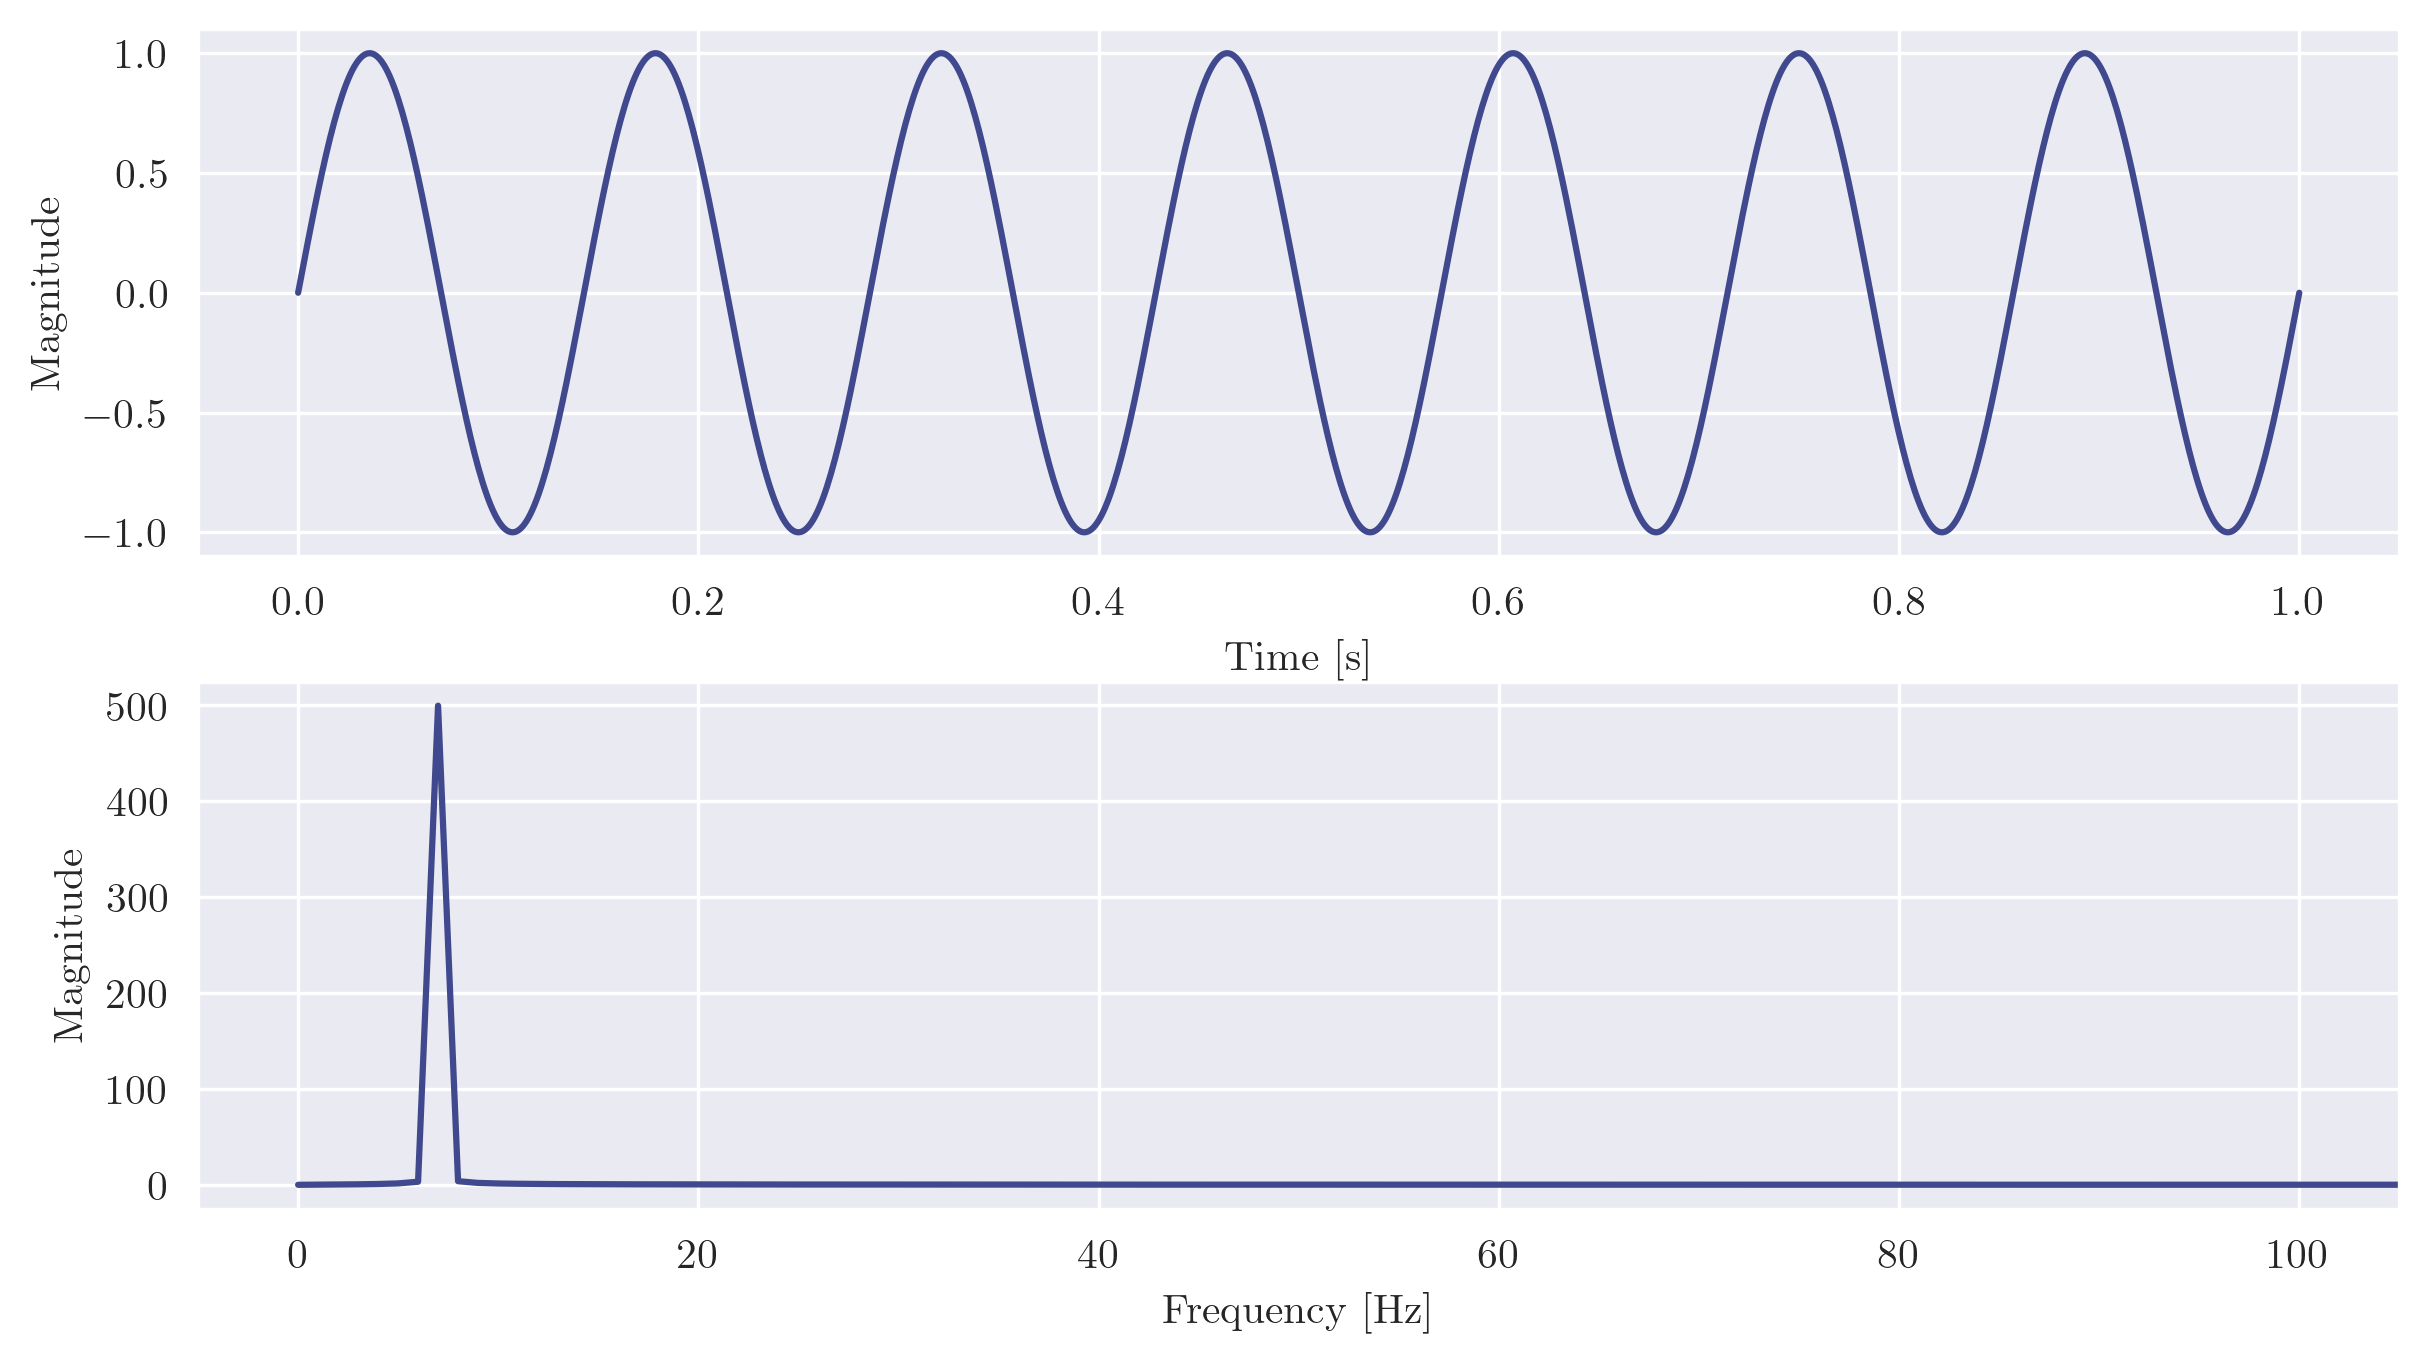
\includegraphics[width=0.8\textwidth]{images/q6_sine7hz.png}
    \caption{Time and frequency views of a 7 Hz sine wave (rendered at
        1 kHz)}
    \label{fig:q6_sine7hz}
\end{figure}

The discrete nature of computer graphics means the visualisation is not truly
continuous, and is actually rendered in timesteps of 1 millisecond. However, for
the purposes of this question, we treat it as continuous to enable comparisons
with subsequent down- and up-sampled signals. The Fourier transform of the
function demonstrates a single peak at 7 Hz, as one would expect.

We now sample the sine wave at 20 Hz, above the Nyquist frequency of 14 Hz.
Therefore, in theory, it should be possible to perfectly reconstruct the
original signal.
\begin{figure}[ht]
    \centering
    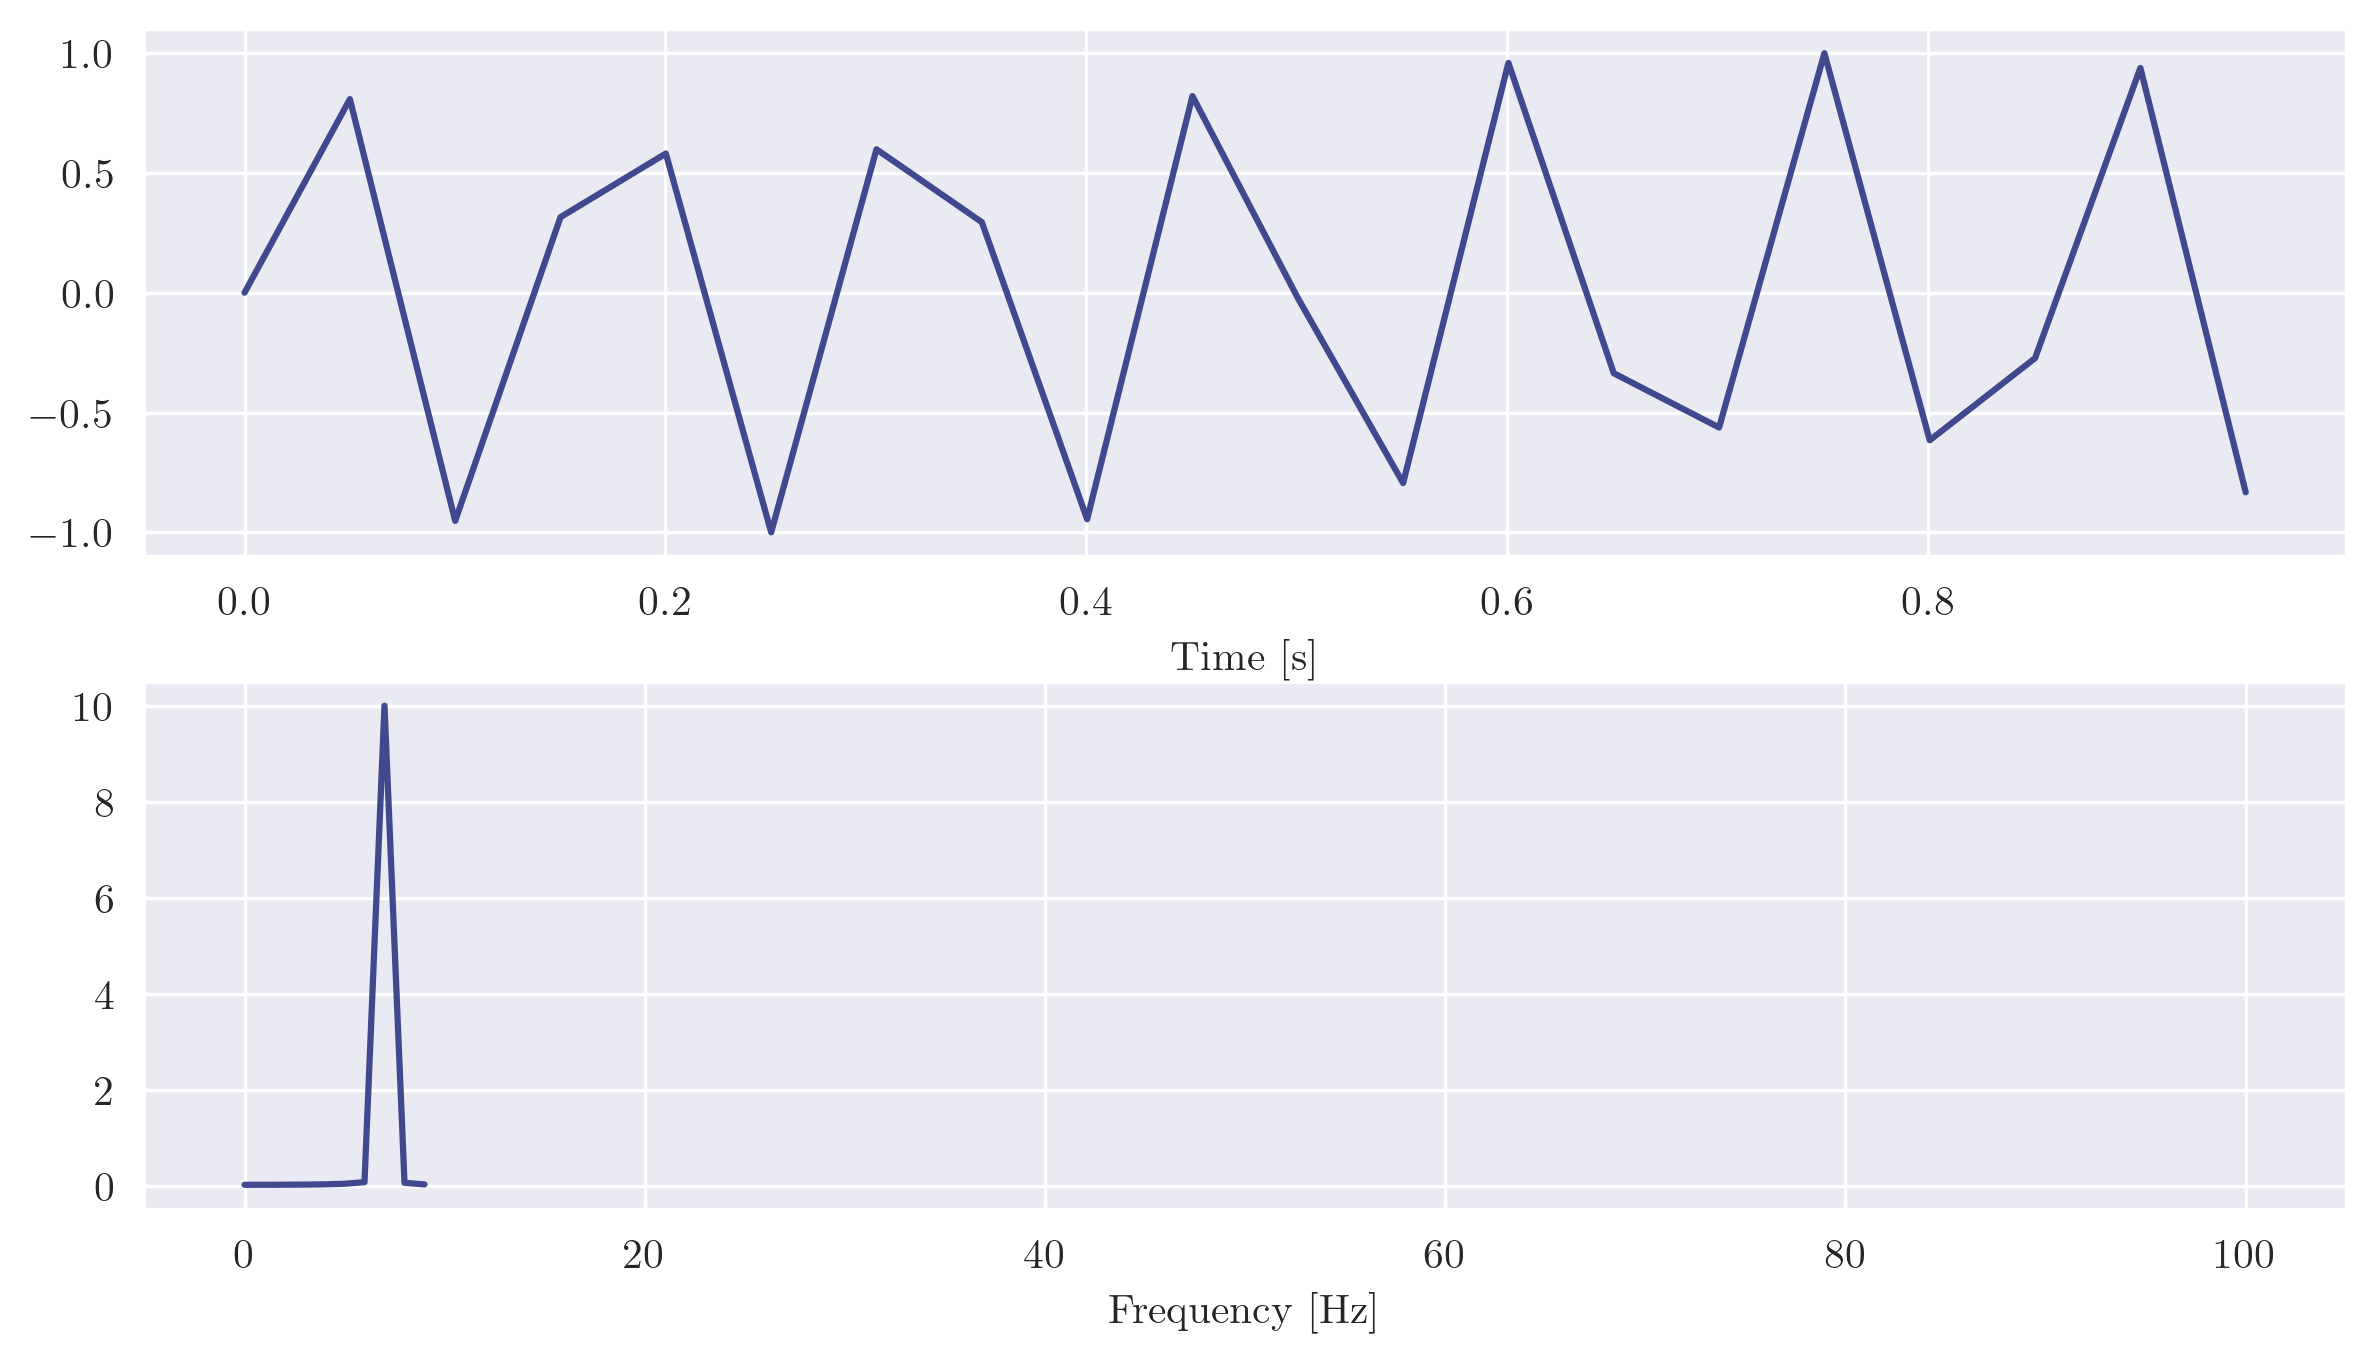
\includegraphics[width=0.8\textwidth]{images/q6_sampled.png}
    \caption{Time and frequency views of the 7 Hz sine wave sampled at 20 Hz}
    \label{fig:q6_sampled}
\end{figure}

In the Fourier domain of Figure \ref{fig:q6_sampled}, we observe the same single
peak at 7 Hz, indicating that the signal indeed has not aliased. Yet, linear
interpolation clearly produces an inaccurate reconstruction of the original sine
wave.

\newpage

A more accurate reconstruction can be achieved using sinc interpolation, whereby
the sampled signal is convolved with a sinc function in the time domain.
Alternatively, this is equivalent to multiplying the Fourier transform of the
sampled signal by a rectangular window.

As a first step, we up-sample the sampled signal from 20 Hz to 80 Hz by padding
three zeros between each sampled value. This produces the following result:

\begin{figure}[ht]
    \centering
    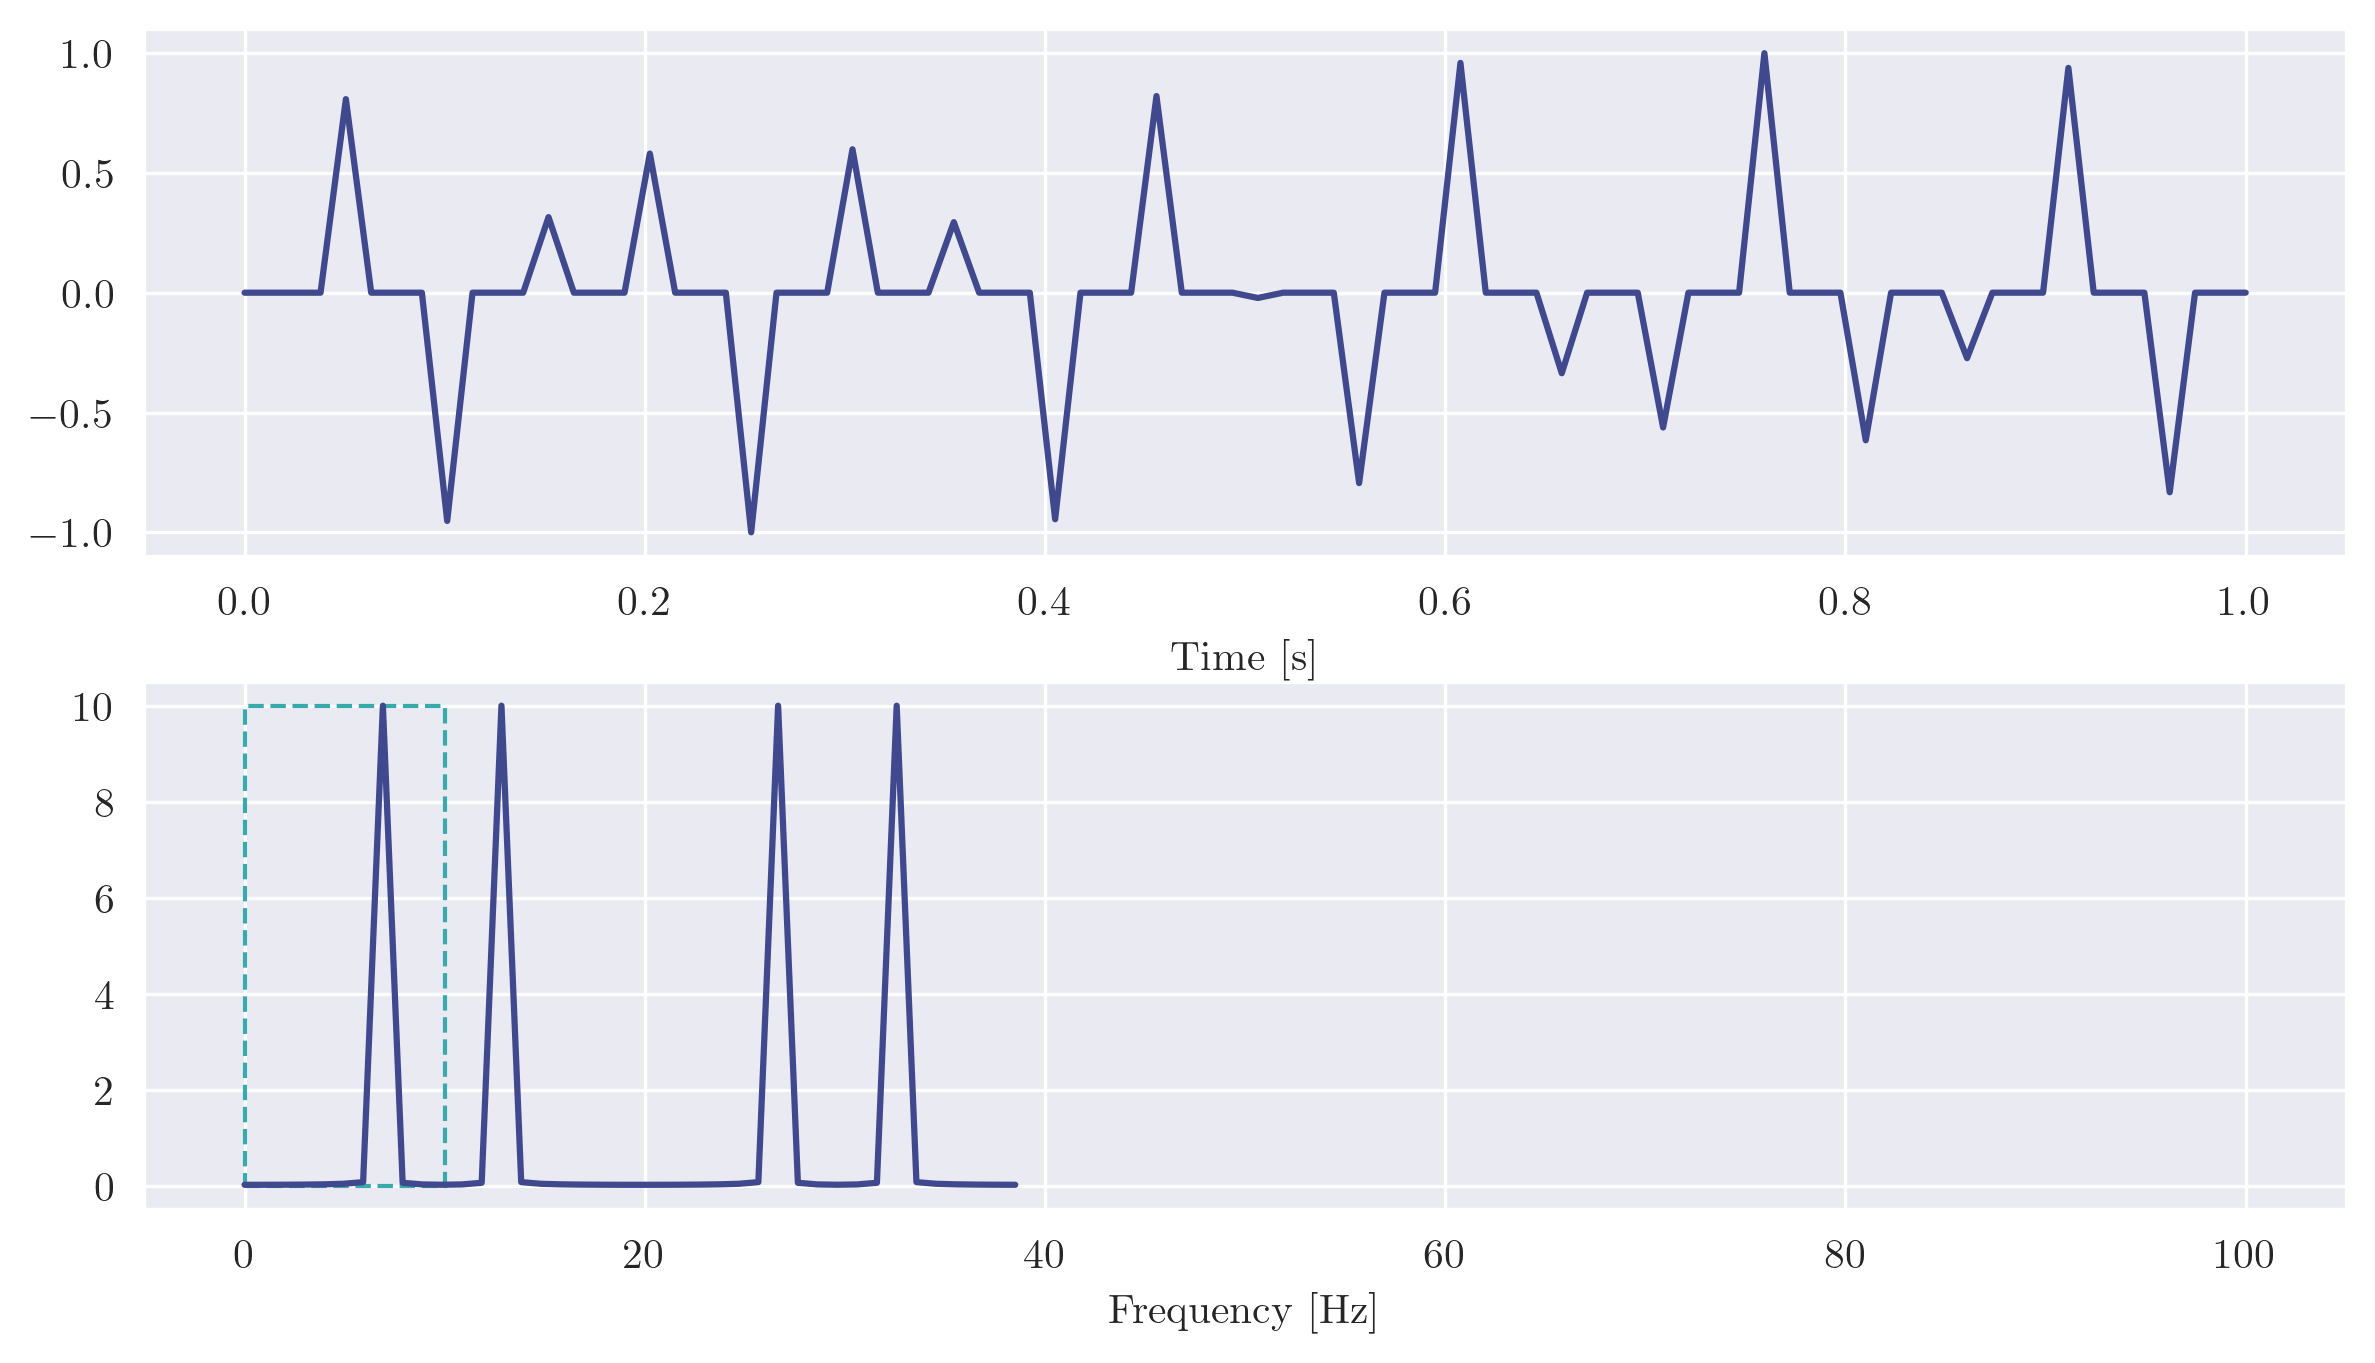
\includegraphics[width=0.8\textwidth]{images/q6_intermediate.png}
    \caption{Time and frequency views of the intermediate upsampled signal}
    \label{fig:q6_intermediate}
\end{figure}

Evidently, upsamping by zero padding has introduced three new peaks in the
Fourier domain, corresponding to the number of zeros padded between each value.
To remove these peaks, we multiply the signal by a rectangular window to filter
out all peaks except the desired 7 Hz peak (and its negative counterpart). The
positive half of this window is indicated in Figure \ref{fig:q6_intermediate}.

To restate, this is equivalent to convolution with a sinc function in the time
domain, and produces the sinc-interpolated signal presented in Figure
\ref{fig:q6_upsampled}.

\begin{figure}[ht]
    \centering
    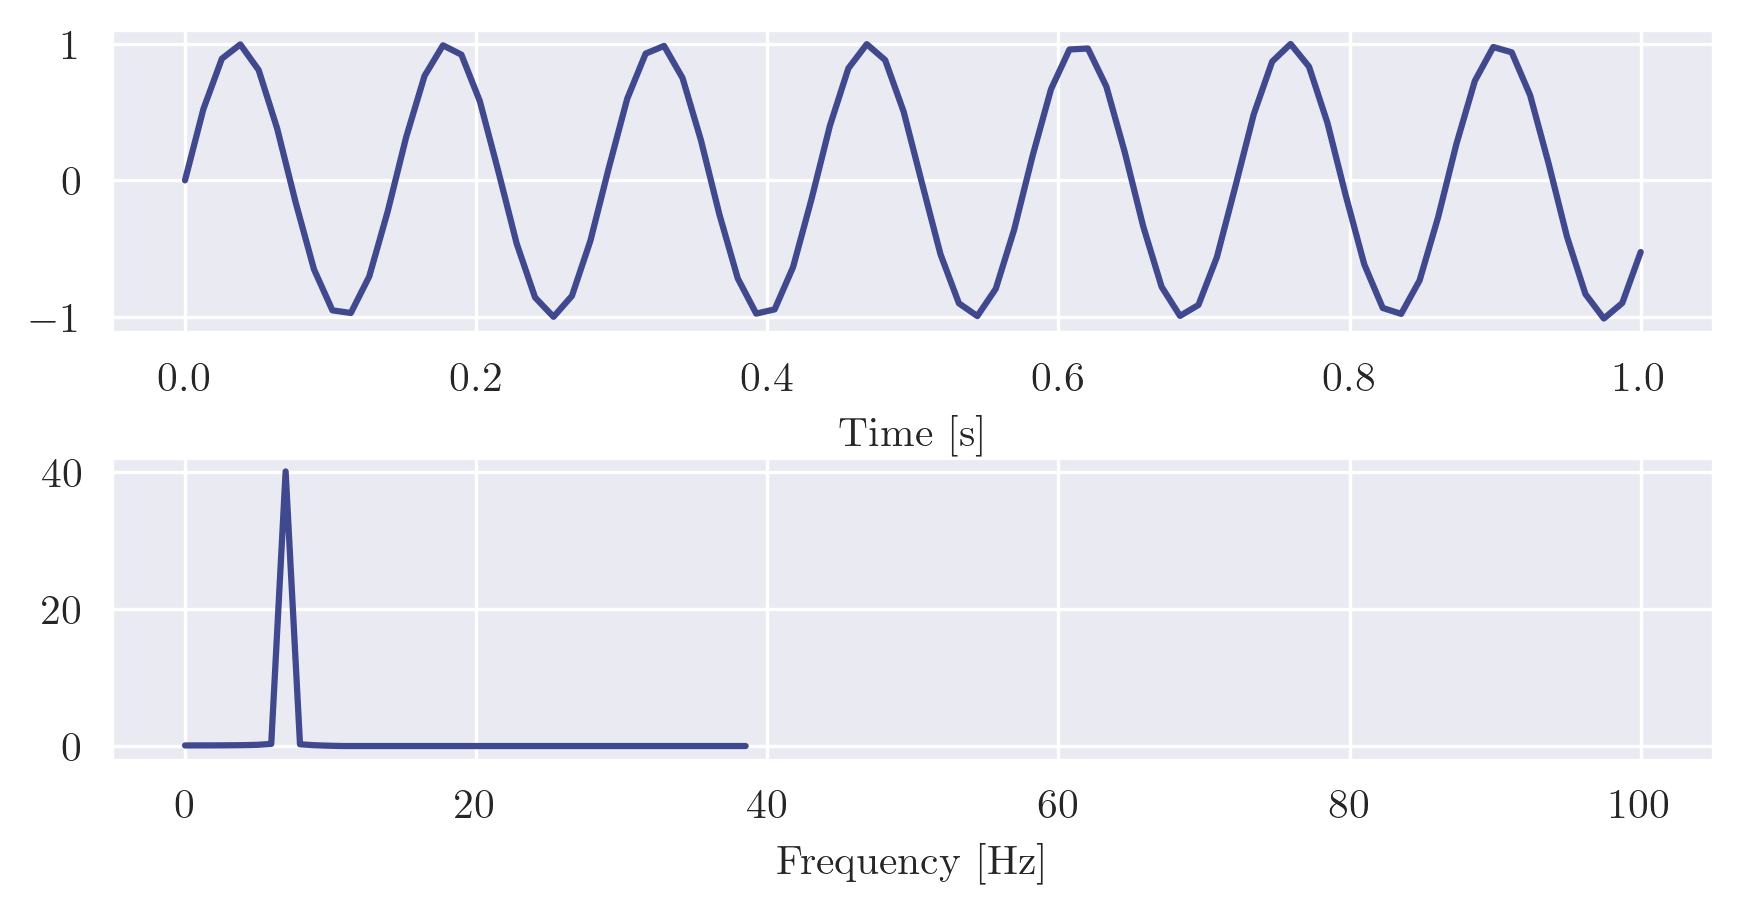
\includegraphics[width=0.8\textwidth]{images/q6_interpolated.png}
    \caption{Time and frequency views of the 80 Hz sinc interpolated signal}
    \label{fig:q6_upsampled}
\end{figure}

Though still not a perfect reconstruction (which we could improve by padding
with more zeros), it is much improved over the linear interpolation of Figure
\ref{fig:q6_sampled}.

\newpage
\section*{Question 7}
\fakesection{7}

As an alternative to sinc interpolation, a signal sampled above the Nyquist
frequency can be interpolated by zero-padding its DFT, then inverse transforming
back to the time domain. To compare this with sinc interpolation, we consider
the same 7 Hz sine wave sampled at 20 Hz.

Consider the Fourier transforms of the sampled and sinc interpolated signals
from Question 6.

\begin{figure}[ht]
    \centering
    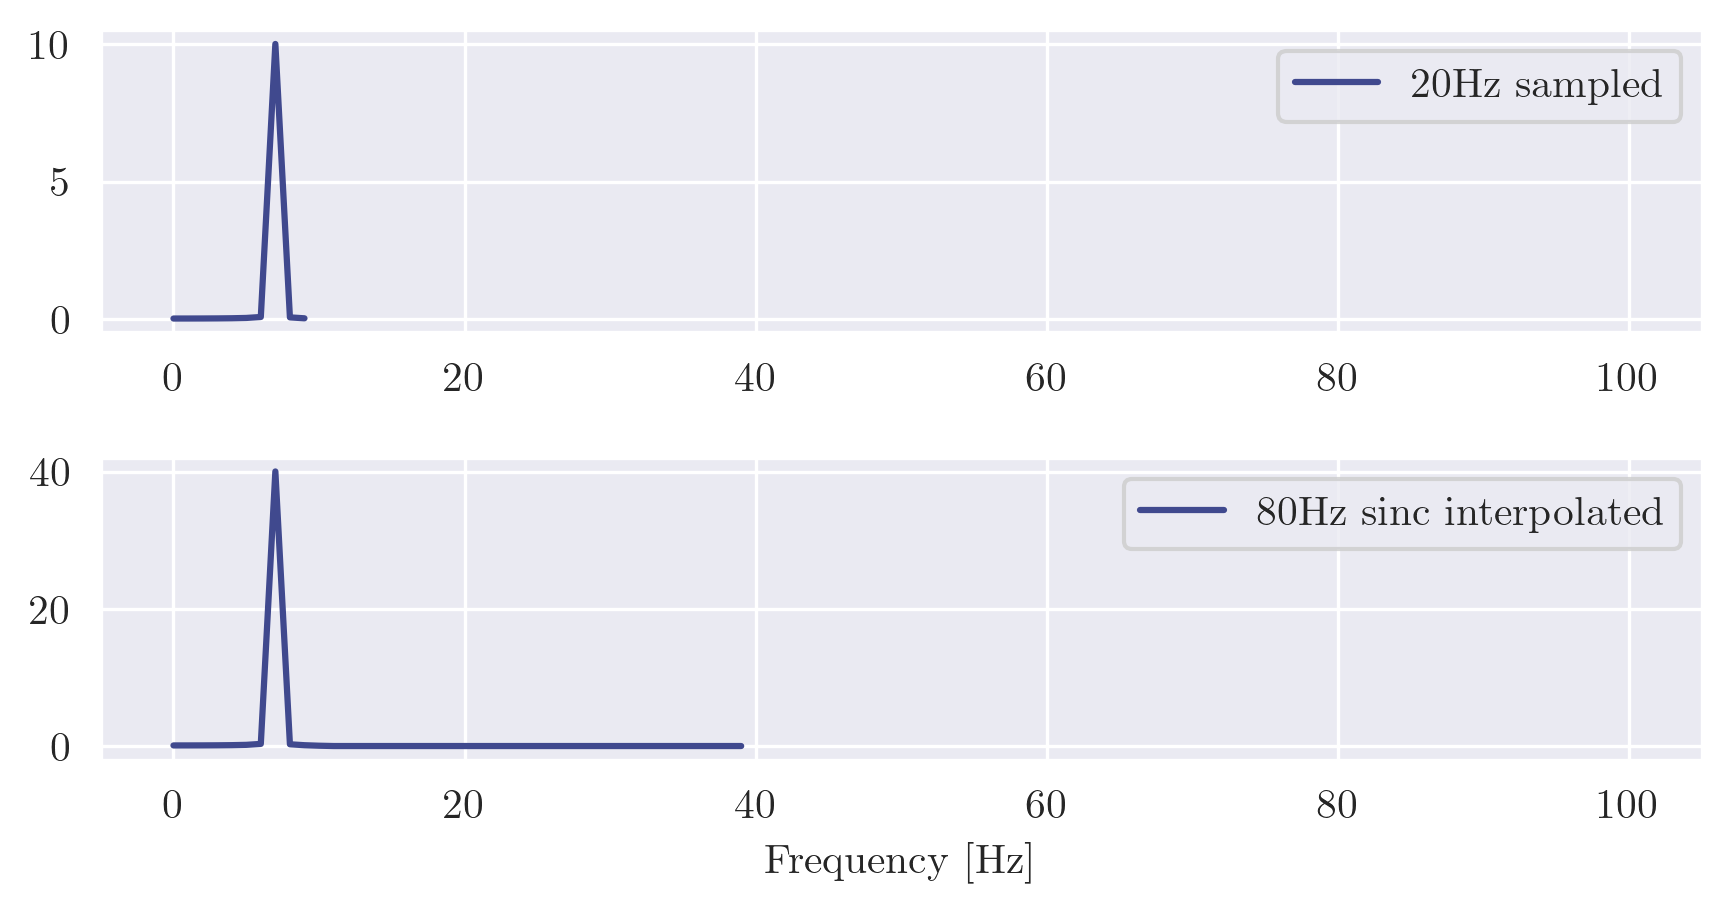
\includegraphics[width=0.8\textwidth]{images/q7_freqcompare.png}
    \caption{Frequency comparison: 20 Hz sampled signal and 80 Hz sinc
        interpolated signal}
    \label{fig:q7_freqcompare}
\end{figure}

The Fourier transform of the 20 Hz sampled signal has a positive bandwidth of
10 Hz (and an equal negative bandwidth, the sum corresponding with the sampling
frequency). The 80 Hz interpolated signal has a positive bandwidth of 40 Hz.
The only difference between them is the length of the (approximately) zero
magnitude tail. Therefore, it should be possible to recreate the interpolation
by zero-padding the Fourier transform of the sampled signal to the desired
length, in both the positive and negative frequencies. This produces Figure
\ref{fig:q7_upsample}.

\begin{figure}[ht]
    \centering
    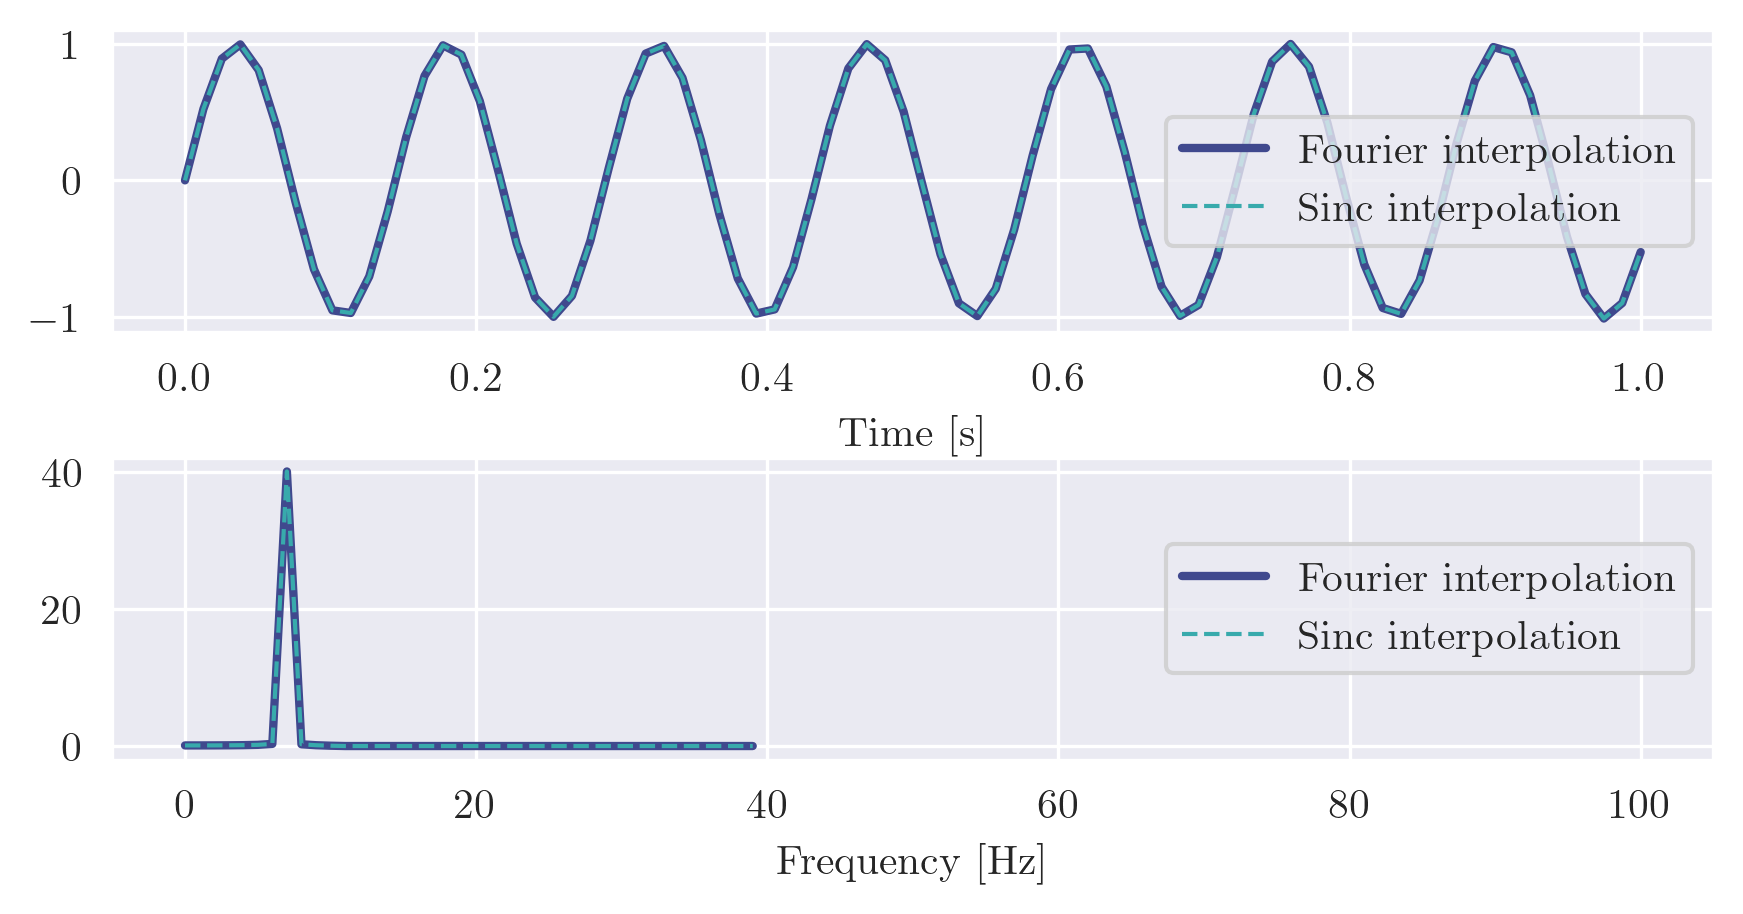
\includegraphics[width=0.8\textwidth]{images/q7_interpolated.png}
    \caption{Time and frequency views of the 80 Hz Fourier interpolated signal}
    \label{fig:q7_upsample}
\end{figure}

As expected, the result is visually indistinguishable from that of sinc
interpolation.

\newpage
\section*{Question 8}
\fakesection{8}

This question aims to use the Fourier transform to determine the duration of a
solar cycle using annual sunspot data from 1700 to 2018. There are several
assumptions associated with this:
\begin{itemize}
    \item the solar cycle is approximately sinusoidal;
    \item the sampling rate of the data is 1 year;
    \item the Nyquist effects are negligible in the data; and
    \item the data has a DC gain; i.e. a non-variable number of sunspots
          occuring each year.
\end{itemize}
Given these assumptions hold, the following analysis should find the average
number of years in the solar cycle. We begin by observing the annual sunspot
data, presented in Figure \ref{fig:q9_timeseries}.

\begin{figure}[ht]
    \centering
    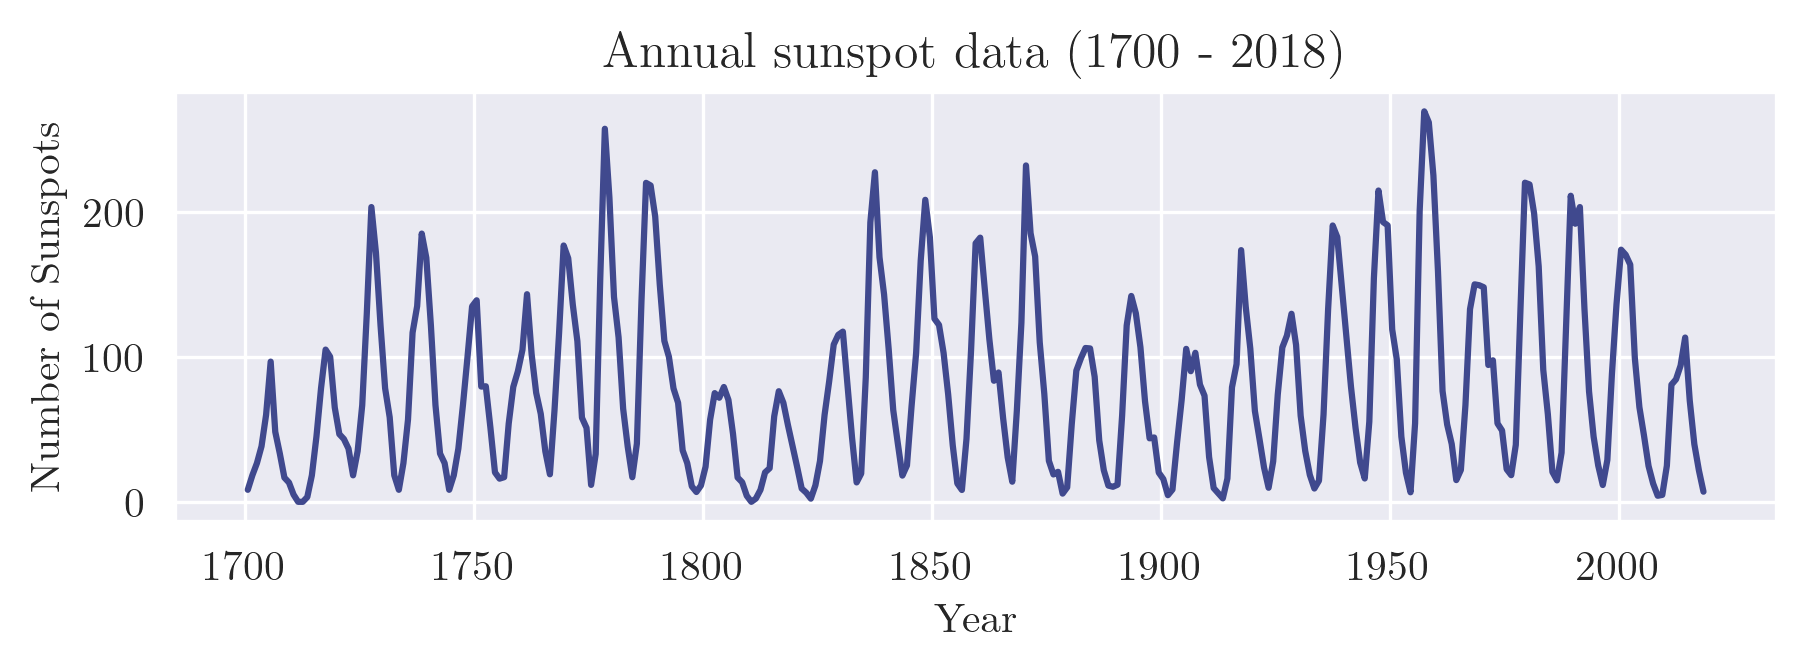
\includegraphics[width=0.9\textwidth]{images/q8_timeseries.png}
    \caption{Annual sunspot data from 1700 to 2018}
    \label{fig:q9_timeseries}
\end{figure}

The data appears to demonstrate two superposed cyclic trends: one of
approximately 10 year period, and another of approximately 80 year period. We
will use the DFT to examine this.

\begin{figure}[ht]
    \centering
    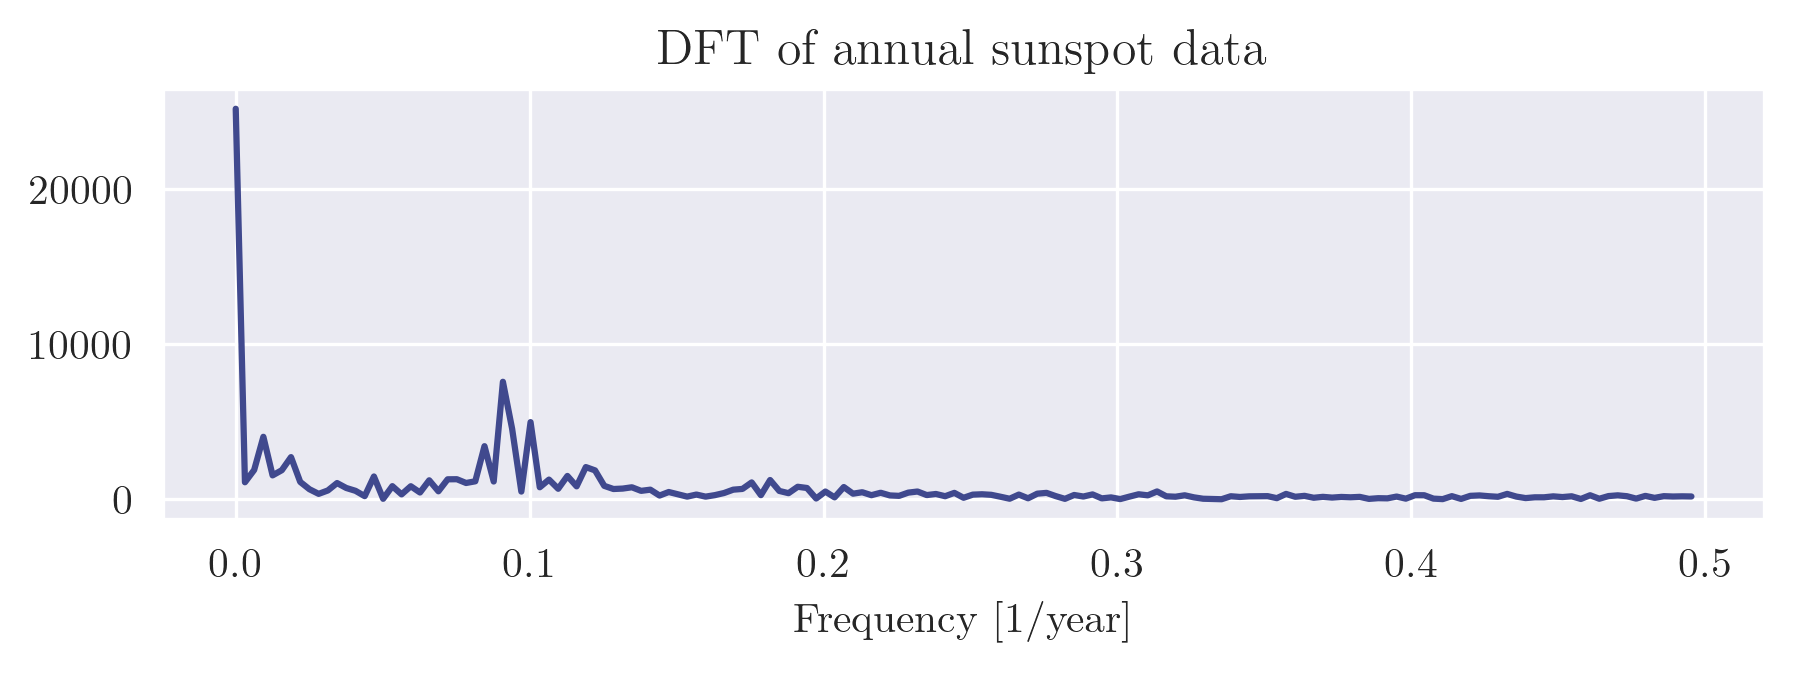
\includegraphics[width=0.9\textwidth]{images/q8_rawdft.png}
    \caption{Fast Fourier transform applied to the annual sunspot data}
    \label{fig:q8_rawdft}
\end{figure}

Taking the DFT of the data, we find validation of the DC gain assumption, and
not much else due to the relative magnitude of the DC gain. To address this, it
is necessary to remove the DC gain by subtracting the mean of the data from the
entire series. Doing so and repeating the DFT, we find the result of Figure
\ref{fig:q8_nodcdft}.

\newpage

\begin{figure}[ht]
    \centering
    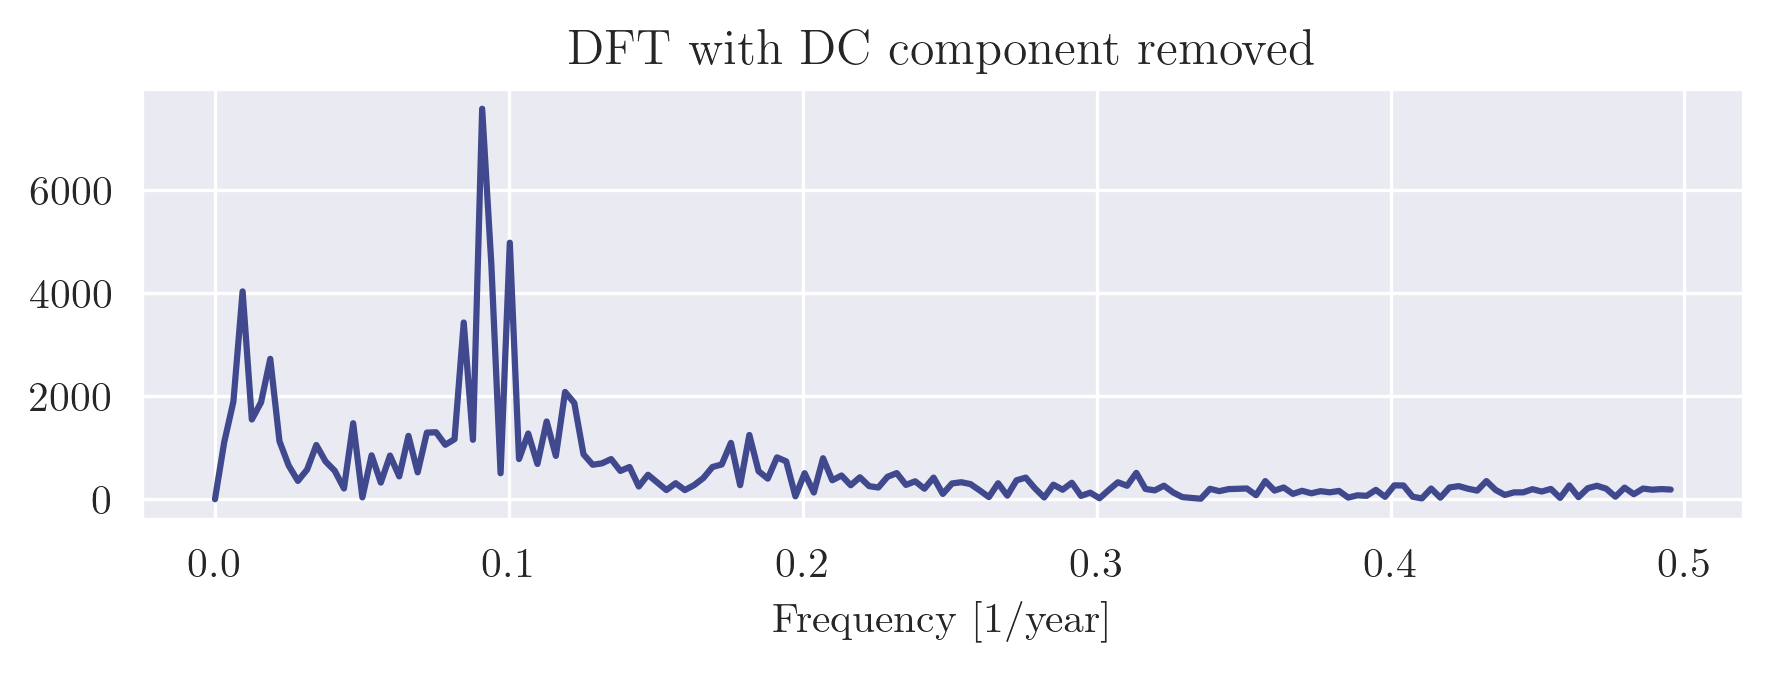
\includegraphics[width=0.85\textwidth]{images/q8_nodcdft.png}
    \caption{Fast Fourier transform applied after removing DC gain}
    \label{fig:q8_nodcdft}
\end{figure}

Having removed the DC gain, the other features in the data become much more
apparent. We now turn our attention to the possibility of spurious components
in the DFT due to the truncation of the series before the first and after the
last years in the data. To investigate this, we apply the rectangular, Hann and
Blackman windows to the time series data and compare the resulting Fourier
transforms.

\begin{figure}[ht!]
    \centering
    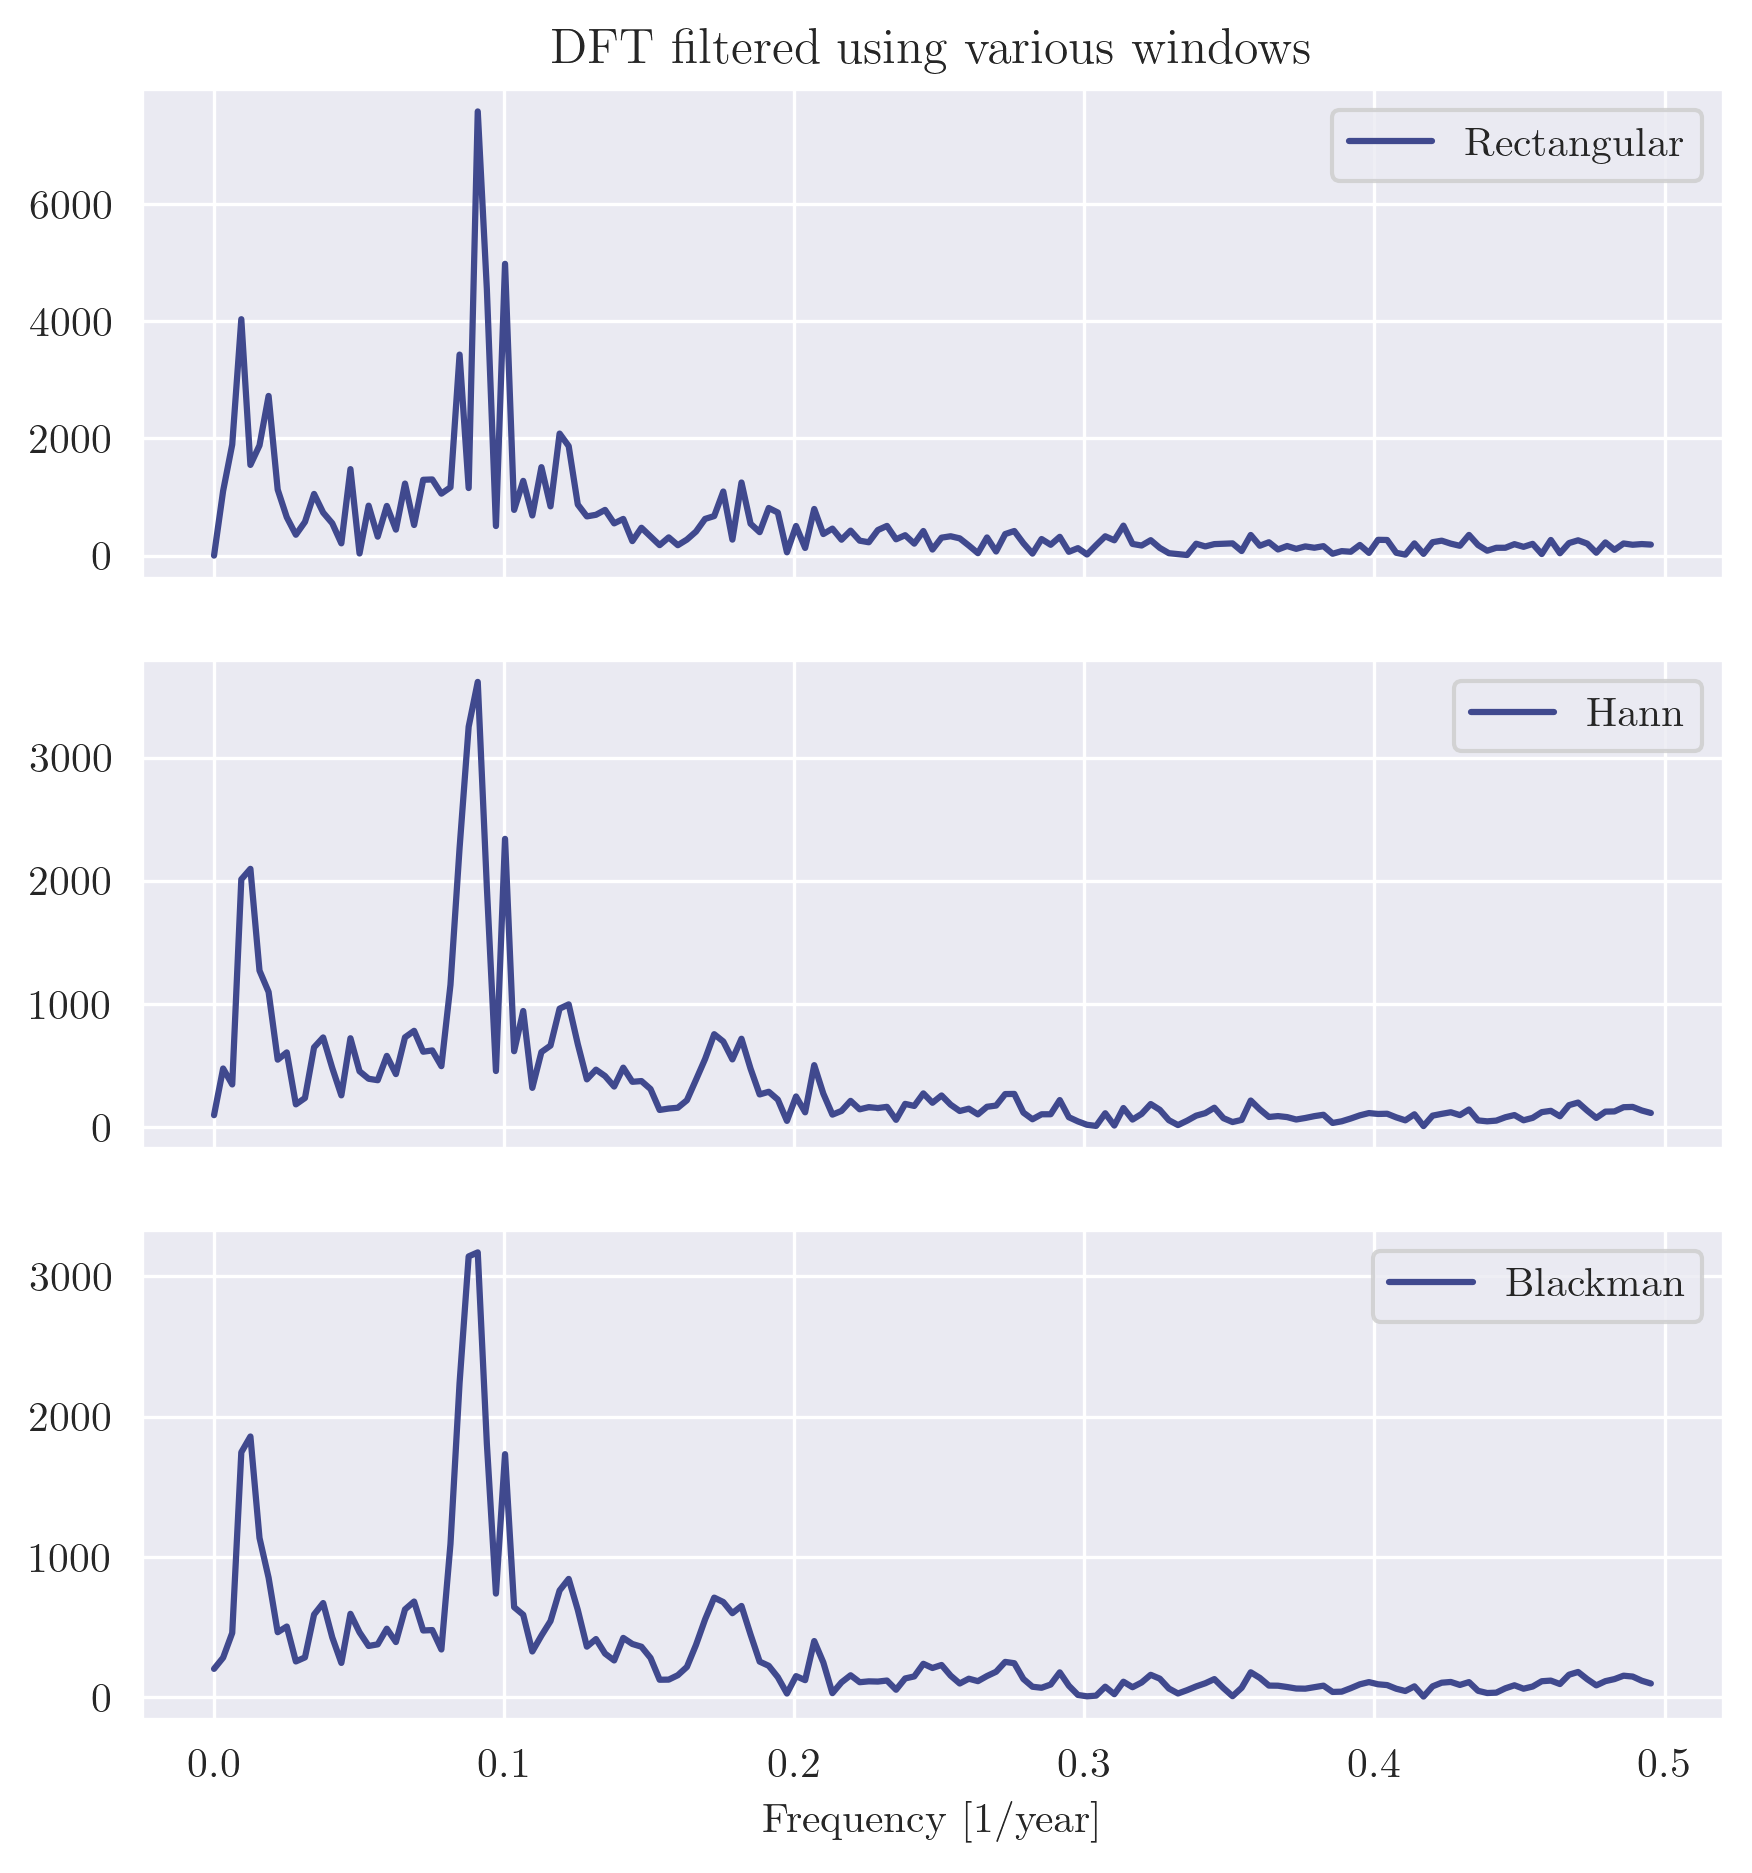
\includegraphics[width=0.85\textwidth]{images/q8_windowed.png}
    \caption{Effects of rectangular, Hann and Blackman windows}
    \label{fig:q8_windows}
\end{figure}

\newpage

Addressing the windows in order, we first observe that applying the rectangular
window has no visible effect. This is because the original series, truncated to
the range 1700 to 2018, is effectively multiplied by a rectangular window around
the same range. Hence, applying the rectangular window again is redundant.
Meanwhile, the Hann and Blackman windows emphasise the peaks in the Fourier
transform and suppress the other frequencies; the effect is more pronounced for
the Blackman window than the Hann window. As we are after the maxima in the
Fourier transform, we prefer the Blackman window over the other two.

To precisely locate the maxima, we will refer to the coarse and fine search
algorithm described by Rife and Boorstyn\footnote{D. C. Rife and R. R. Boorstyn,
``Single-tone parameter estimation from discrete-time observations,"
\textit{IEEE Trans. Inf. Theory}, vol. IT-20, no. 5, pp. 591-598, Sep., 1974.}.
However, whereas the Rife and Boorstyn algorithm finds a single global maximum,
we are interested in identifying two peaks. Therefore, we will apply the
algorithm twice separately on the frequency ranges $[0, 0.5]$ and $[0.5, 1.5]$.

The Rife and Boorstyn algorithm searches for a maximum of $|A(\omega)|$, where
$A(\omega)$ is defined as
\begin{align*}
    A(\omega) = \frac{1}{N} \sum_{n=0}^{N-1} Z_n \exp(-jn\omega T)
\end{align*}
in which $Z_n$ is the $n$-th observation of the discrete signal $Z$ of total
length $N$, and the frequency $\omega$ is defined between 0 and $\omega_s$, the
sampling frequency\textsuperscript{1}. The sampling period $T$ is the inverse of
$\omega_s$. The coarse search evaluates $|A(\omega)|$ at the set of frequencies
$\{\omega_k\}$ defined by:
\begin{align*}
    \omega_k = \frac{2\pi k}{MT}, \quad k = 0,1,2,\ldots,M-1
\end{align*}
where $M$ is $2N$, $4N$, or $8N$\textsuperscript{1}. This is equivalent to
evaluating the DFT of the set $\{\bar{Z}_n\}$\textsuperscript{1}:
\begin{align*}
    \bar{Z}_n = \begin{cases}
        (M/N)Z_n, & n = 0,1,2,\ldots,N-1 \\
        0,        & n = N,N+1,\ldots,M
    \end{cases}
\end{align*}
Hence, the coarse search can be performed by constructing the set
$\{\bar{Z}_n\}$ and returning the discrete frequency with the largest amplitude
in the DFT of $\{\bar{Z}_n\}$\textsuperscript{1}. Applied to the sunspot data
and using $M=2N$, the coarse search finds the two peaks of interest at
frequencies 0.089 and 0.011 per year, corresponding with periods of
approximately 11.2 and 91.1 years.

The fine search performs a narrow uni-directional sweep of the region around the
coarse result. Let us denote an arbitrary coarse search result as $\omega_l$.
The direction of the sweep depends on the gradient of $|A(\omega_l)|$; if the
gradient of $|A(\omega_l)|$ is positive, the desired maximum is at a value of
$\omega>\omega_l$, else if the gradient of $|A(\omega_l)|$ is negative, the
desired maximum $\omega<\omega_l$\textsuperscript{1}.

As recommended by Rife\footnote{D. C. Rife, ``Digital tone parameter estimation
in the presence of Gaussian noise," Ph.D. disseration, Polytech. Inst. Brooklyn,
Brooklyn, N.Y., Jun. 1973.}, the fine search iterates in steps of size
$\omega_s/(5N)$. The search terminates when the gradient of $|A(\omega)|$
crosses zero\textsuperscript{2}. Finally, the last two points on either side of
the zero are input to the secant root-finding method\footnote{Wikipedia.
``Secant method." Wikipedia.org. https://en.wikipedia.org/wiki/Secant\_method
(accessed Aug. 14, 2023).}. The secant method is considered to have converged
once the difference between successive approximations is less than half the
desired precision; we choose a precision of five decimal places, which will
yield the required three decimal places in the reciprocals.

Applying the fine search to the coarse results from the sunspot data, the peaks
are found at frequencies of approximately 0.01115 and 0.08947 per year, or
equivalently, periods of approximately 11.176 and 89.664 years.

\newpage

Figure \ref{fig:q8_searchresults} presents DFT of the Blackman-windowed signal
with the identified frequencies.

\begin{figure}[ht]
    \centering
    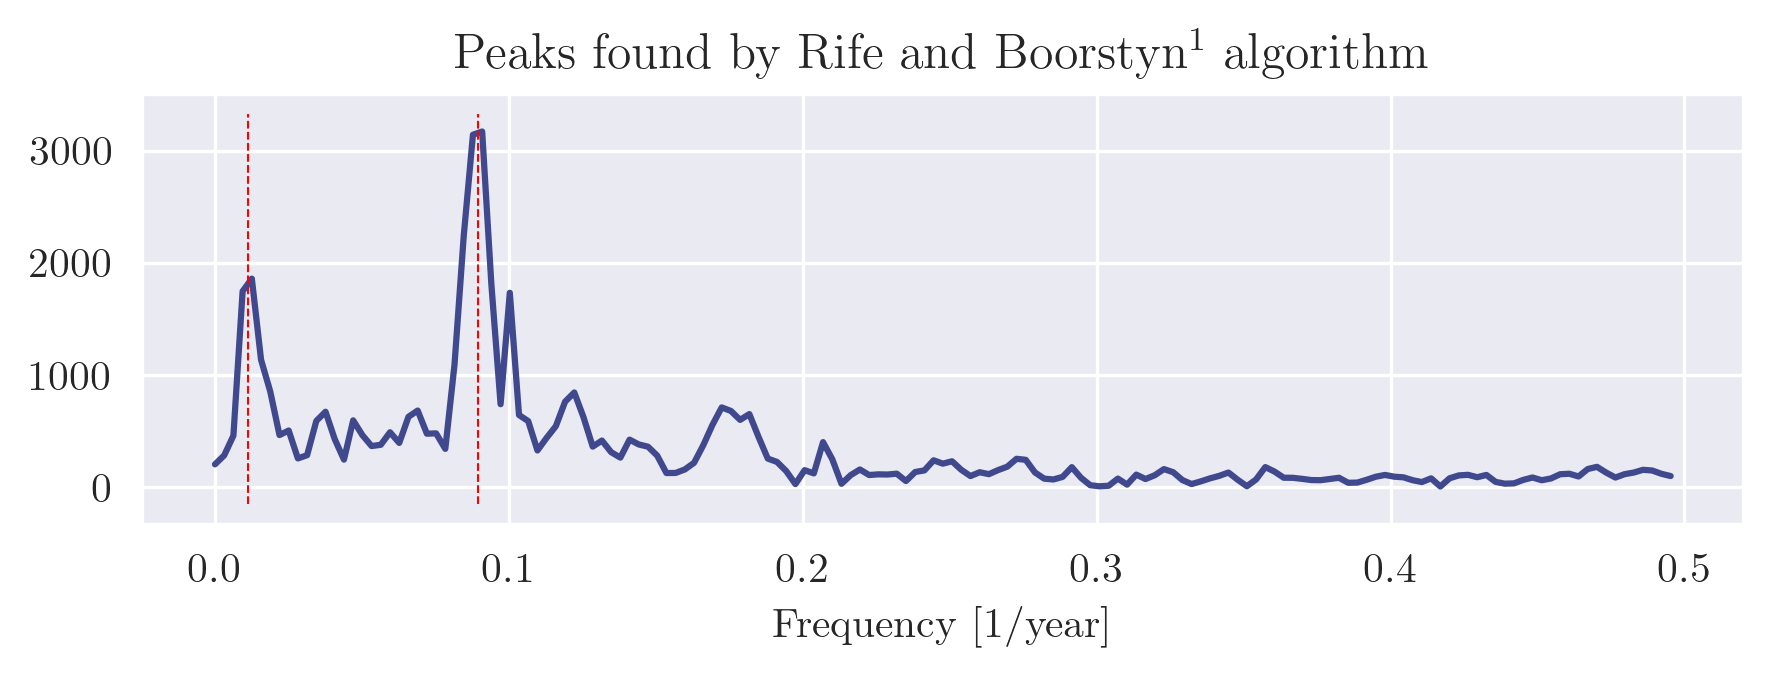
\includegraphics[width=0.8\textwidth]{images/q8_searchresults.png}
    \caption{DFT of Blackman-windowed signal with identified frequencies in red}
    \label{fig:q8_searchresults}
\end{figure}

Notice also how the identified frequencies occur between points of the DFT,
especially evident in the second peak. The Rife and Boorstyn\textsuperscript{1}
algorithm enables higher precision than simply returning the frequency which
produces the largest response in the DFT.

The 11.176-year period in the sunspot data corroborates the general consensus
of a solar cycle period of approximately 11 years\footnote{Wikipedia. ``Solar
cycle.'' Wikipedia.org. https://en.wikipedia.org/wiki/Solar\_cycle (accessed
Aug. 14, 2023).}. However, observations of cycles as short as 9 years or as
long as 14 years have been recorded\textsuperscript{4}, somewhat undermining
the precision of the identified value. Similarly, the 89.664-year feature
corroborates the period of the Gleissberg cycle, which describes an amplitude
modulation of solar cycles with a period between 70 to 100
years\textsuperscript{4}.

The large variance in both sets of observations makes it more difficult to
justify the three decimal point precision from a purely practical standpoint.
Nevertheless, this investigation has proven to be a useful exercise in
applying DSP methods to extract information from real data.

\newpage
\section*{Question 9}
\fakesection{9}

Figure \ref{fig:q9_headings} visualises the ten homing pigeon departure headings
and their average value.

\begin{figure}[ht]
    \centering
    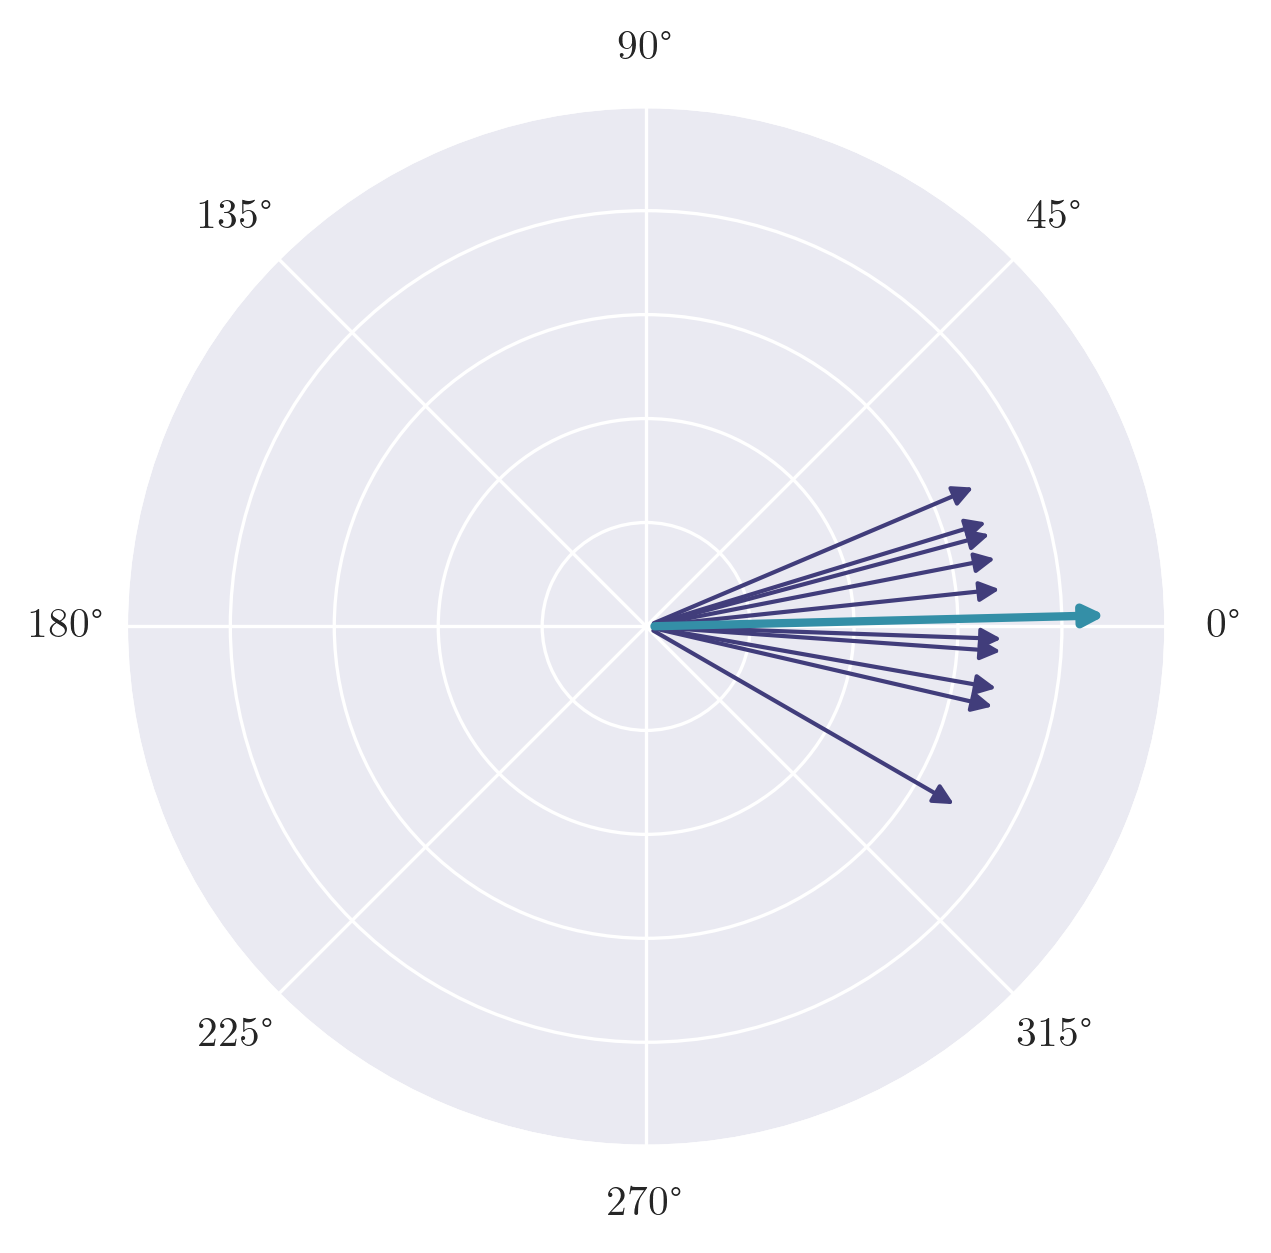
\includegraphics[width=0.6\textwidth]{images/q9_headings.png}
    \caption{Homing pigeon departure headings and average heading}
    \label{fig:q9_headings}
\end{figure}

To calculate the average heading, one might consider naively summing and
dividing the values.
\begin{align*}
    \frac{11+15+350+330+23+347+17+356+6+358}{10} = 181.3^\circ
\end{align*}
In doing so, one quickly realises that the result is exactly in the opposite
direction to the expected average heading, because the headings are distributed
on either side of the 360$^\circ$ modulus angle.

A better method is to convert the headings into complex numbers using polar
($e^{j\theta}$) form, average them, and determine the argument of the result.
For example, for the heading of 11$^\circ$:
\begin{align*}
    e^{j(11\times(\pi/180))} \approx 0.982+j0.191
\end{align*}
We can perform the conversion for each heading and average the real and
imaginary parts separately to obtain the following average heading as a complex
number: $0.964+j0.023$.

Finally, we determine the argument of the complex number and convert from
radians to degrees:
\begin{align*}
    \arctan(\frac{0.023}{0.964}) \approx 0.024 \text{rad} \approx 1.390^\circ
\end{align*}
Hence, we have determined an average heading matching our observation of Figure
\ref{fig:q9_headings}.

%-----------------------
% Code listings
%-----------------------
\newpage
\appendix
\begin{center}
    \LARGE{\textbf{Appendix}}
\end{center}

\section{Code Listings}
\textit{(Starts on the following page)}

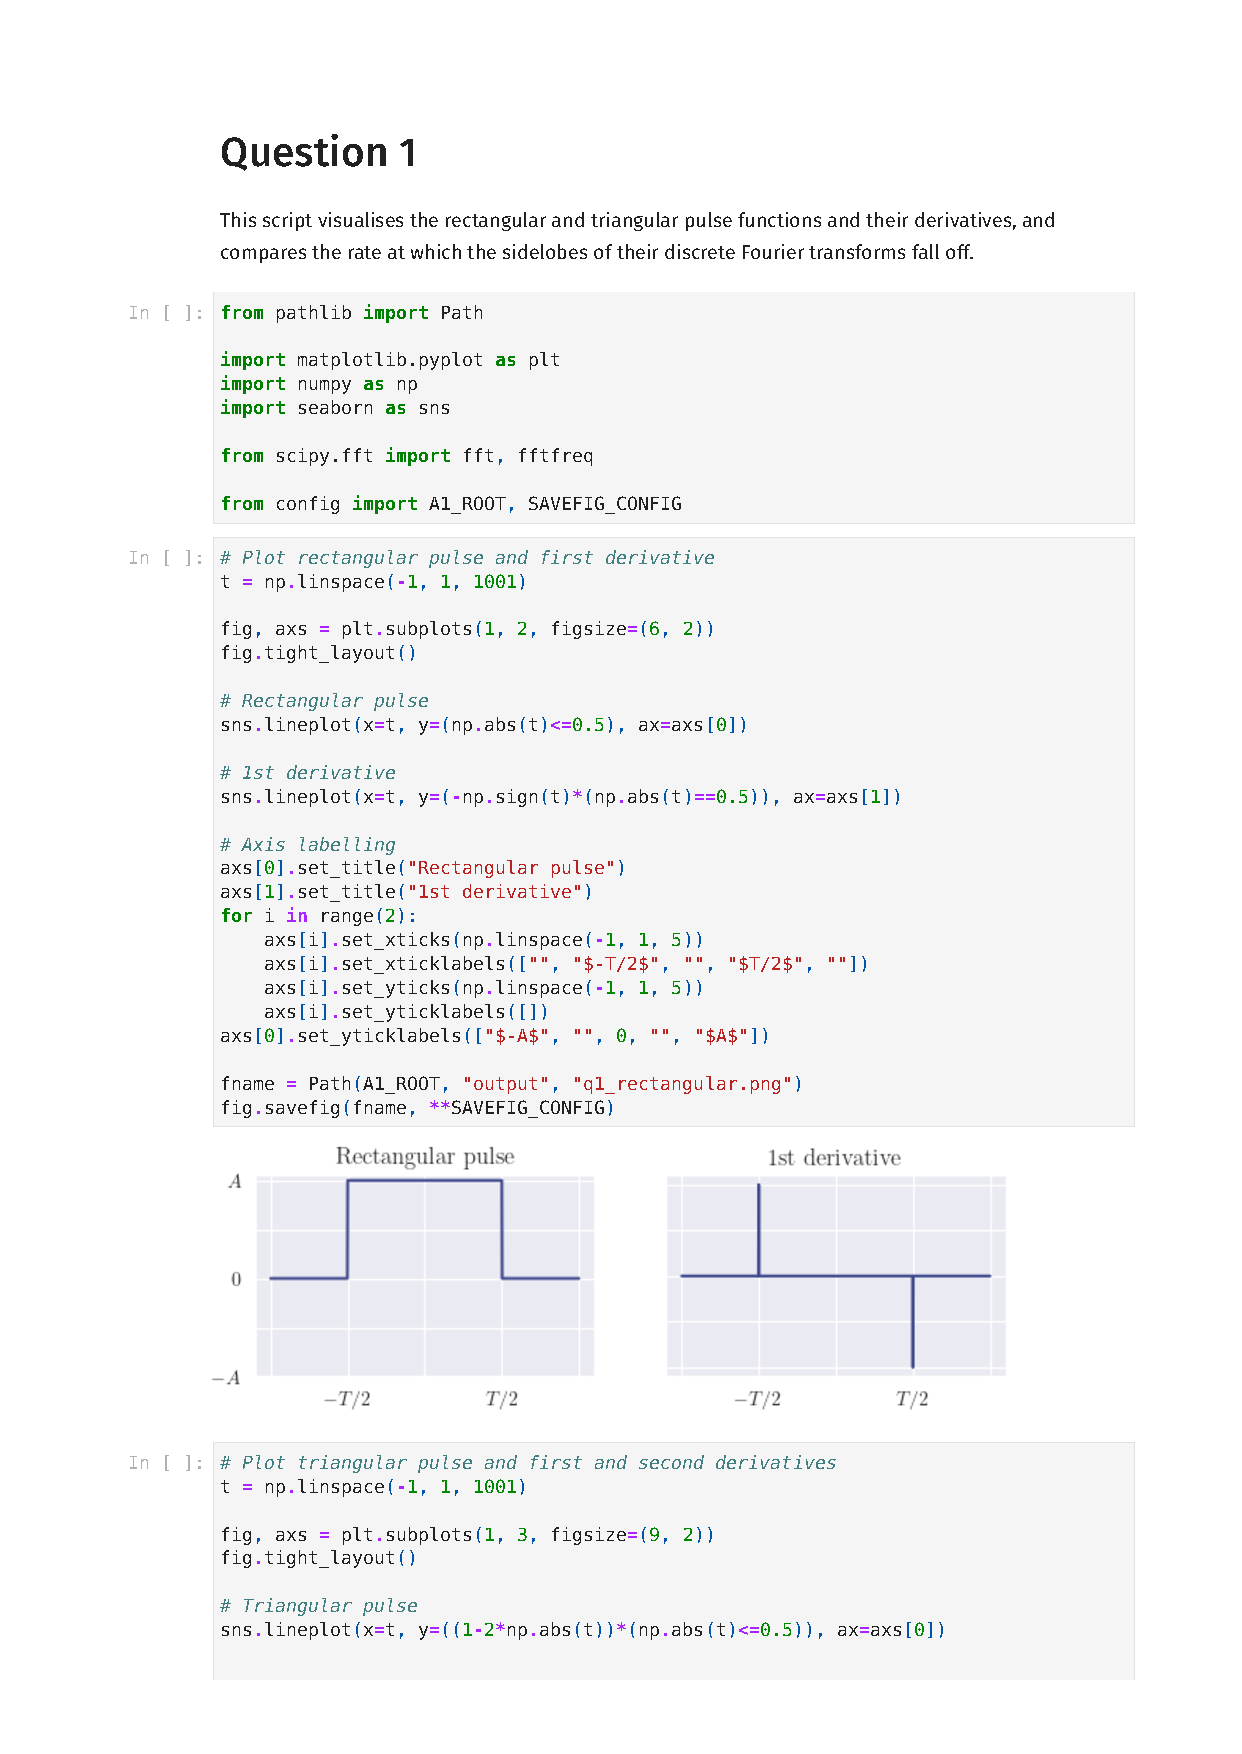
\includepdf[pages=-]{pdfpages/q1_sidelobes.pdf}
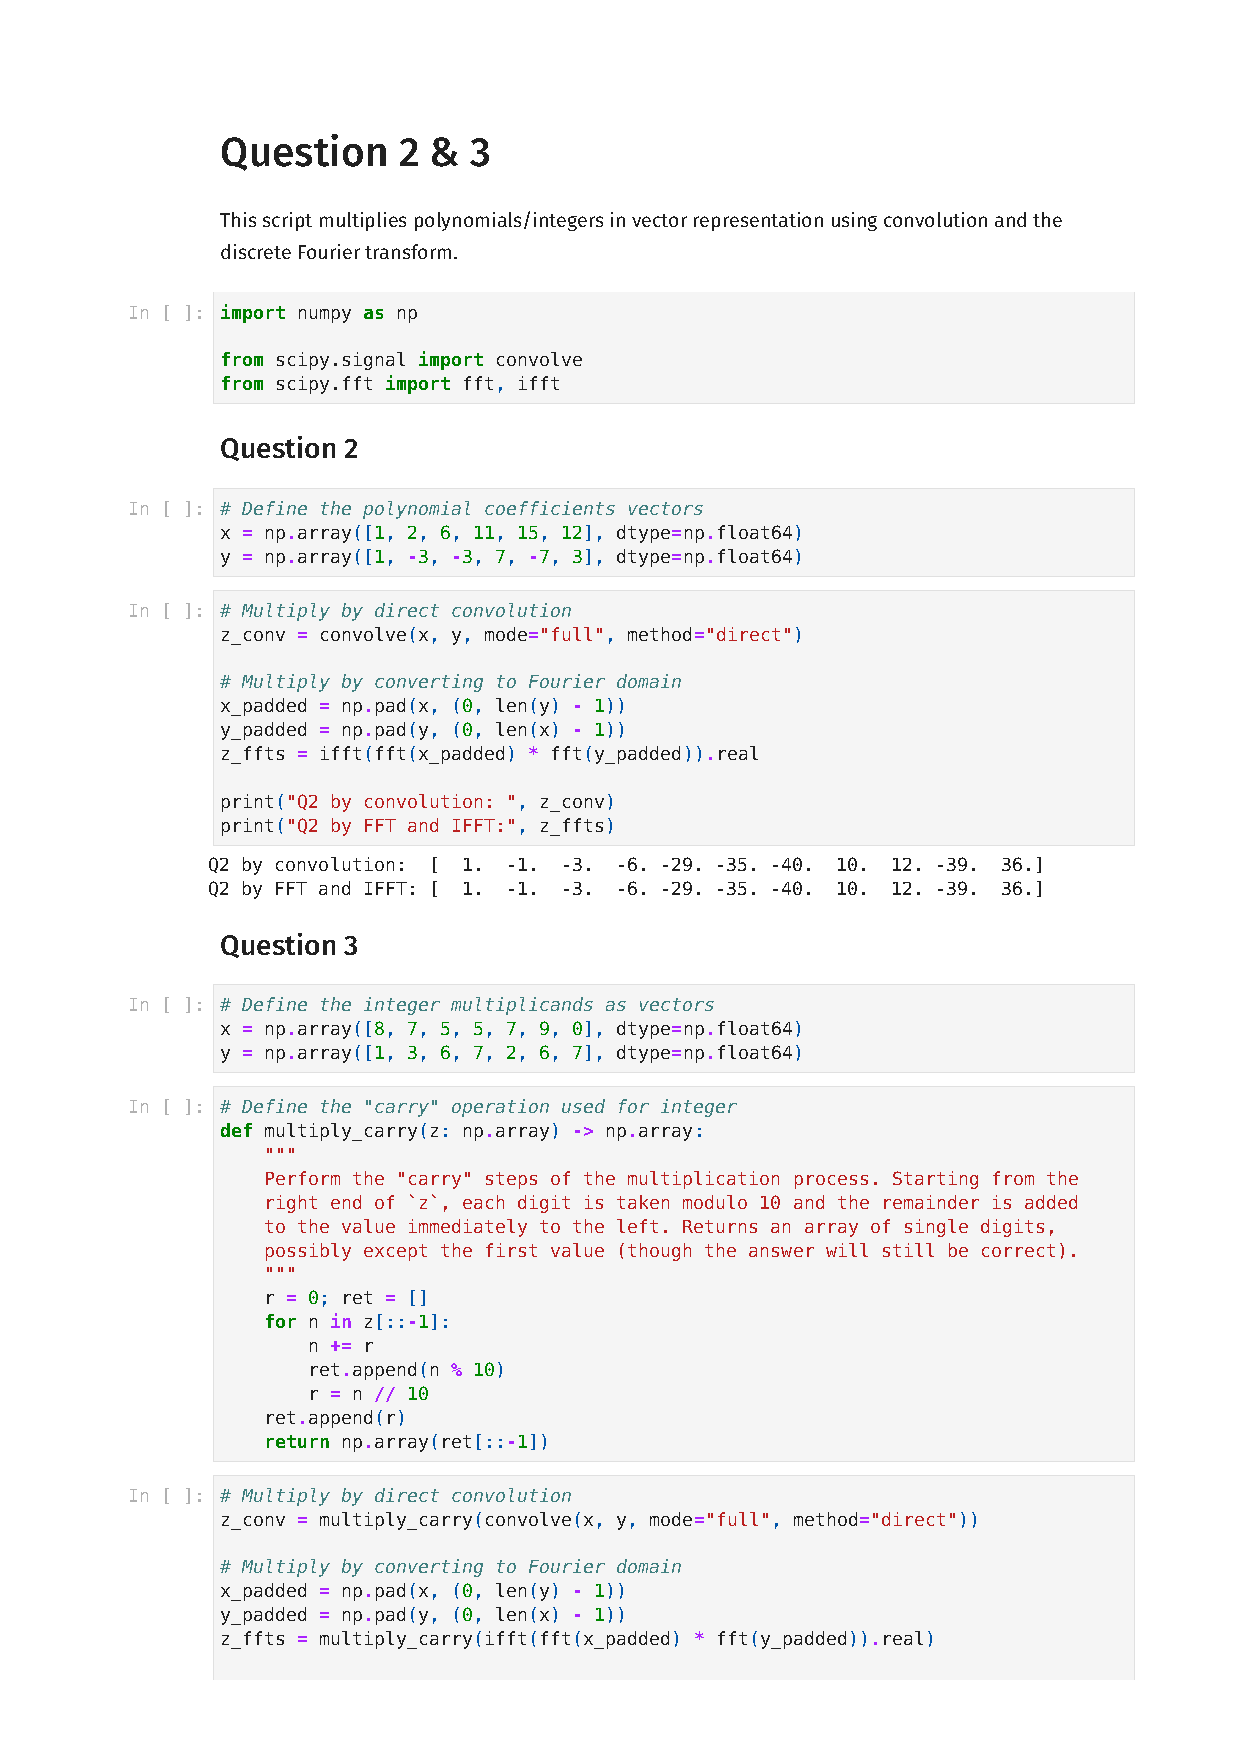
\includepdf[pages=-]{pdfpages/q2_3_multiplying.pdf}
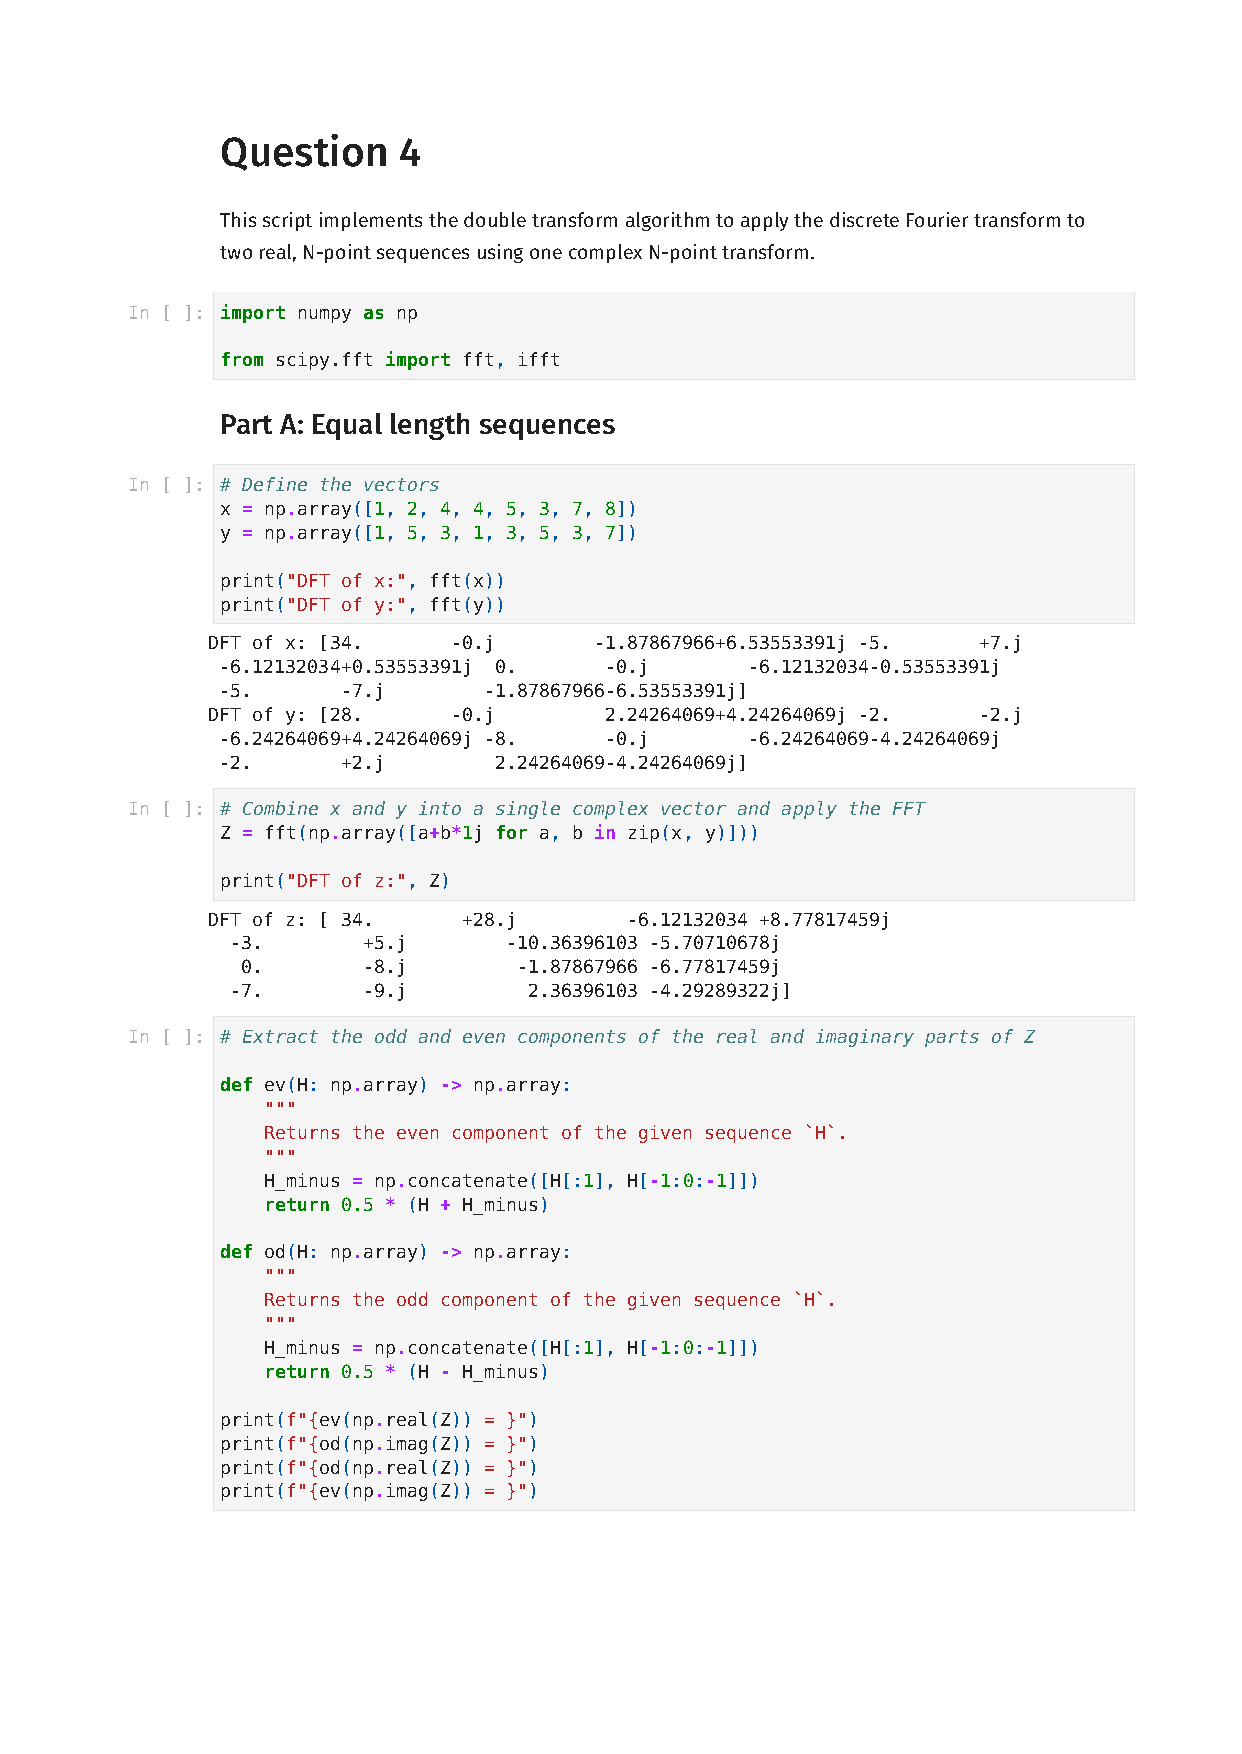
\includepdf[pages=-]{pdfpages/q4_double_transform.pdf}
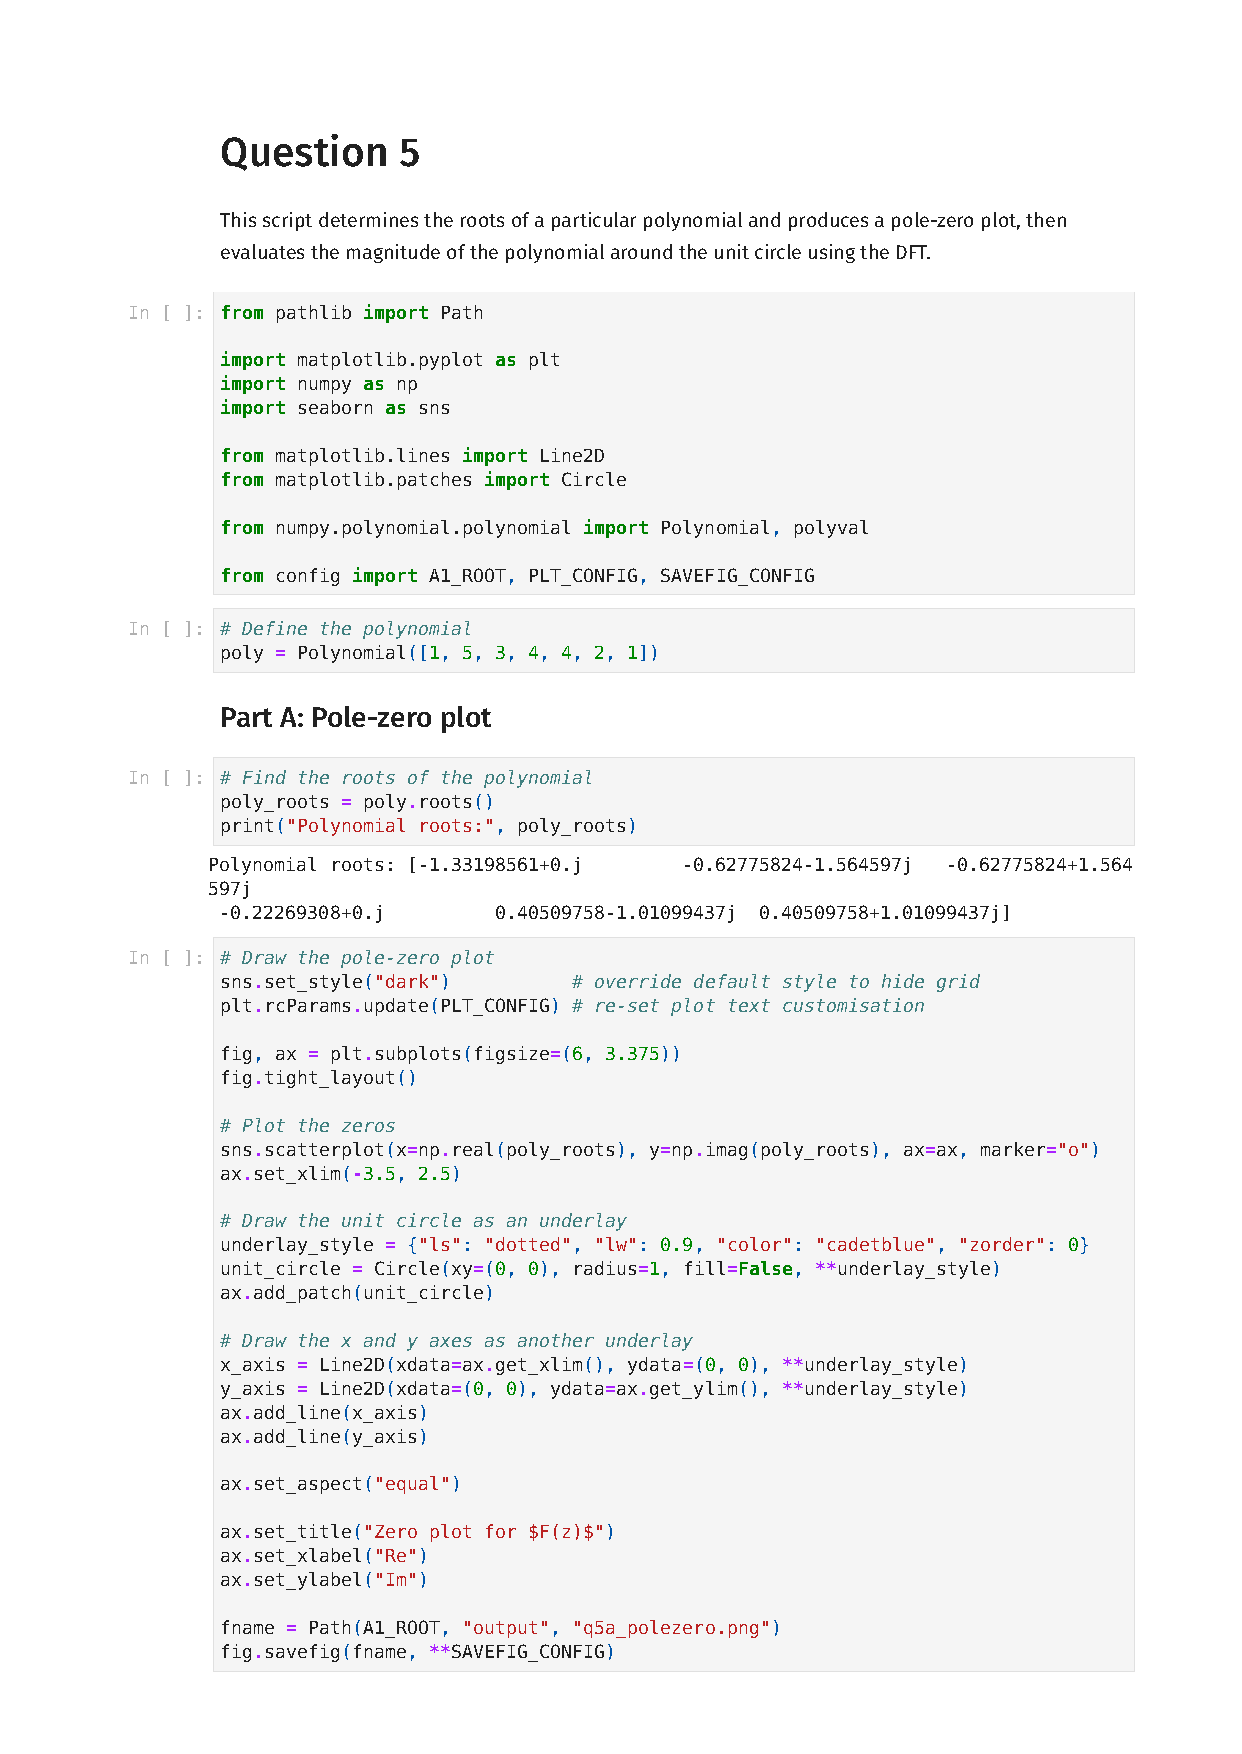
\includepdf[pages=-]{pdfpages/q5_polezero.pdf}
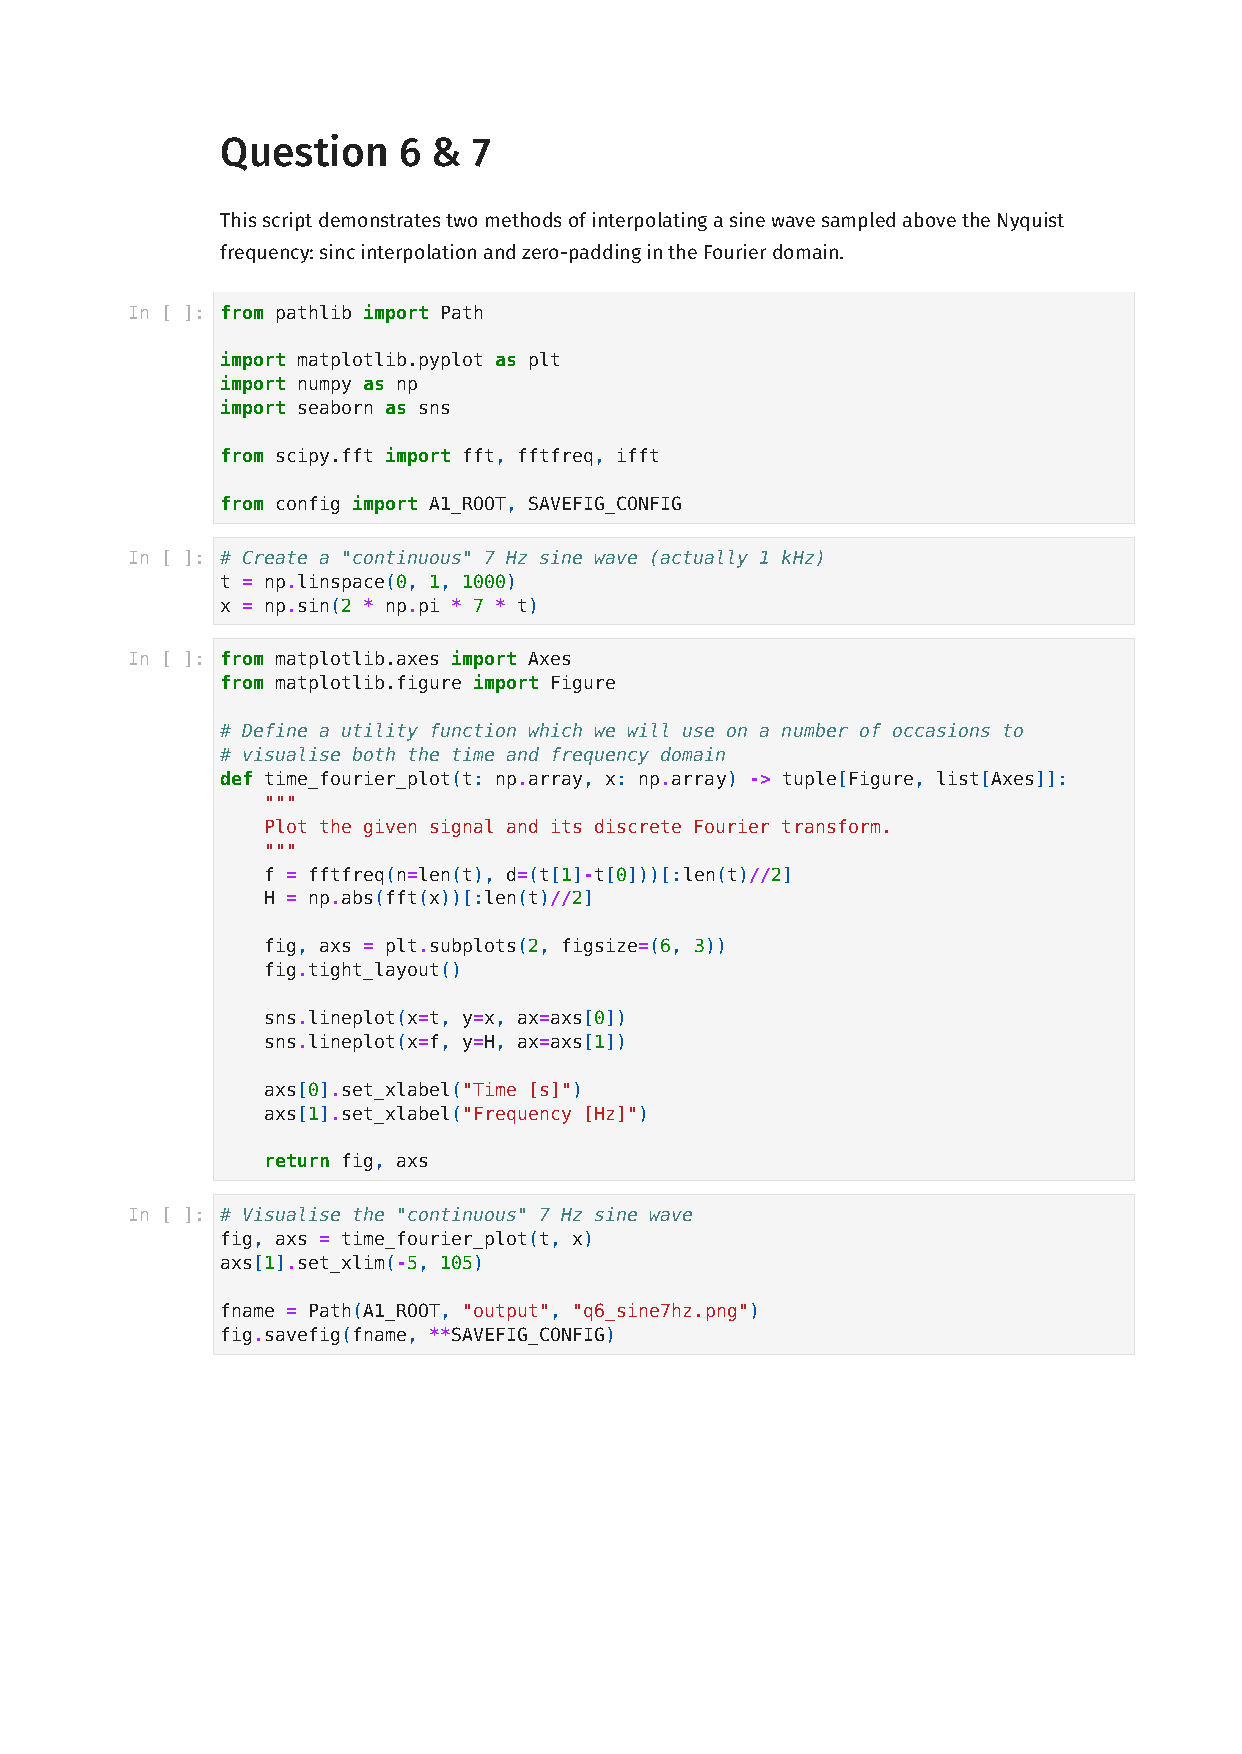
\includepdf[pages=-]{pdfpages/q6_7_interpolation.pdf}
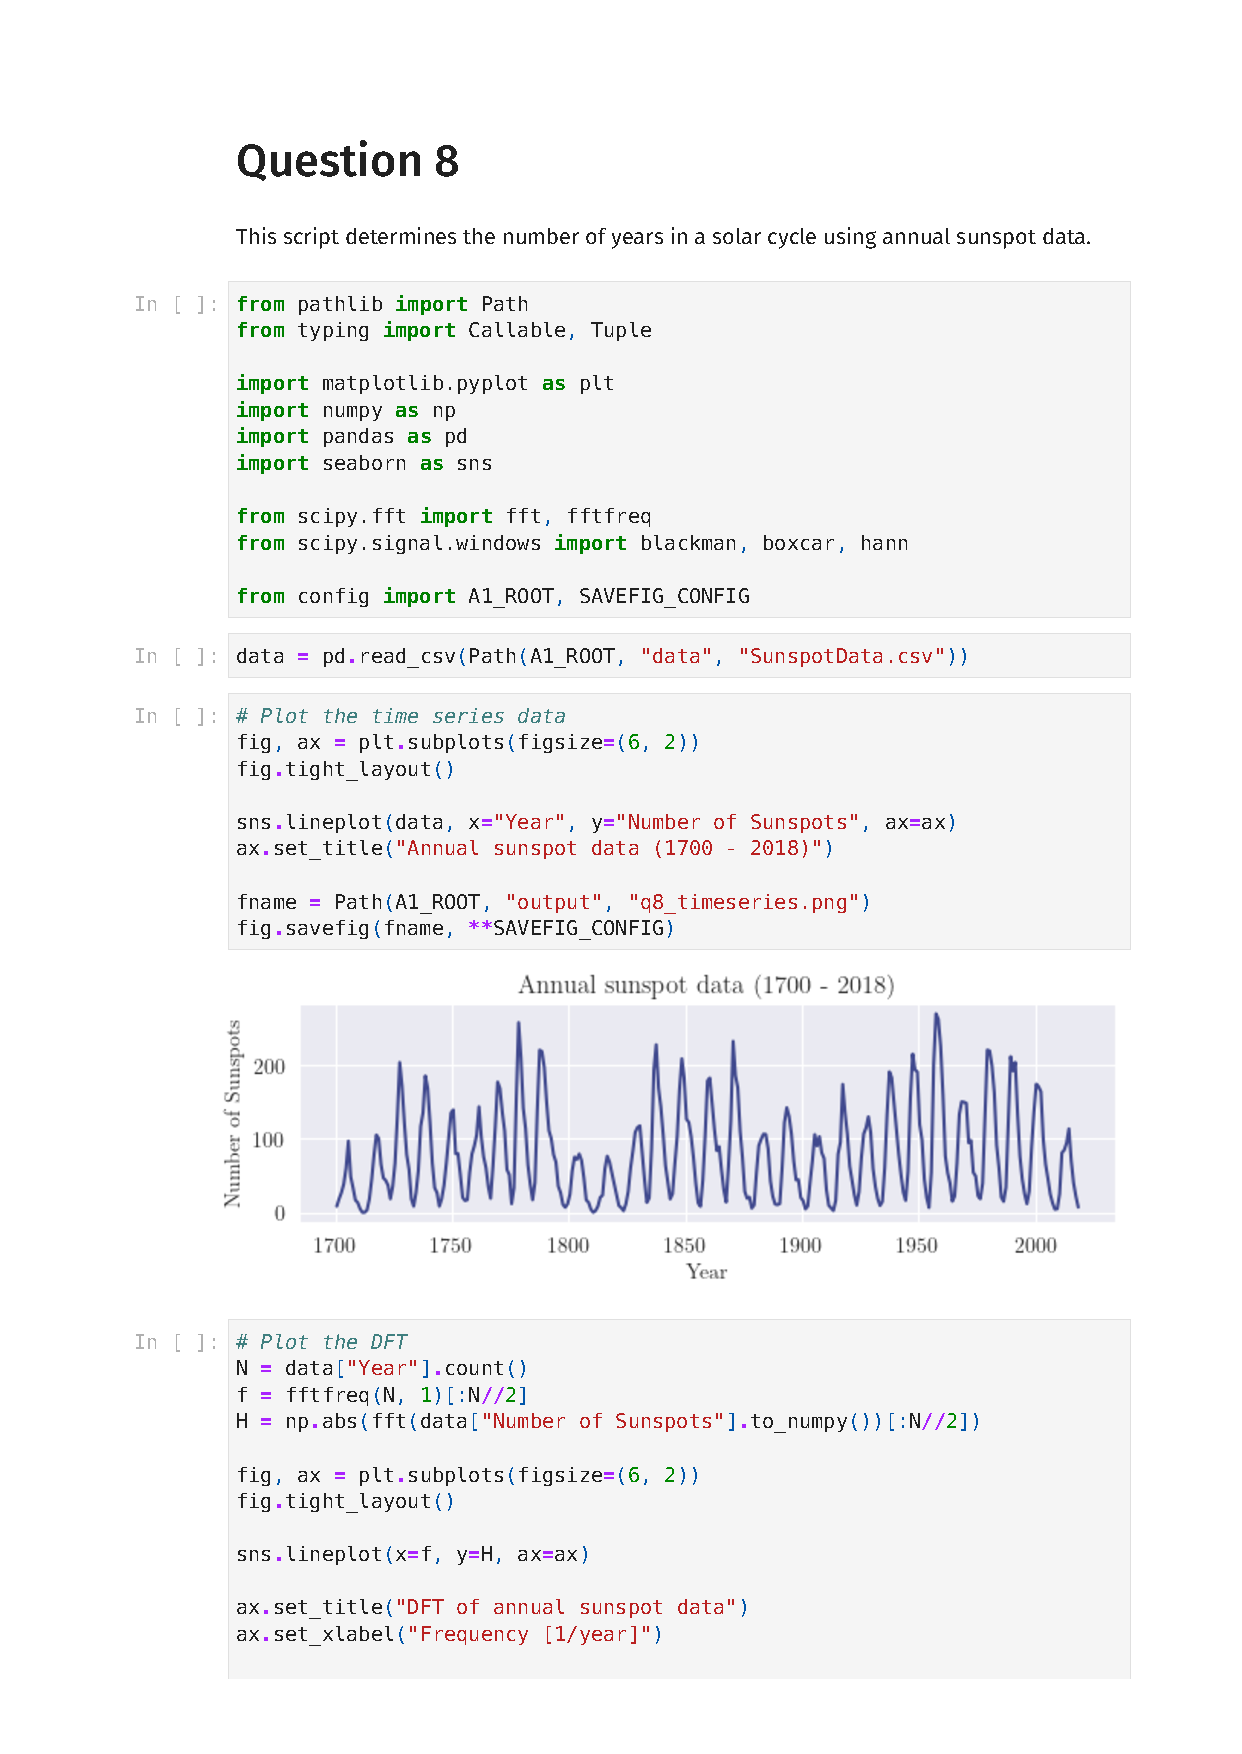
\includepdf[pages=-]{pdfpages/q8_sunspots.pdf}
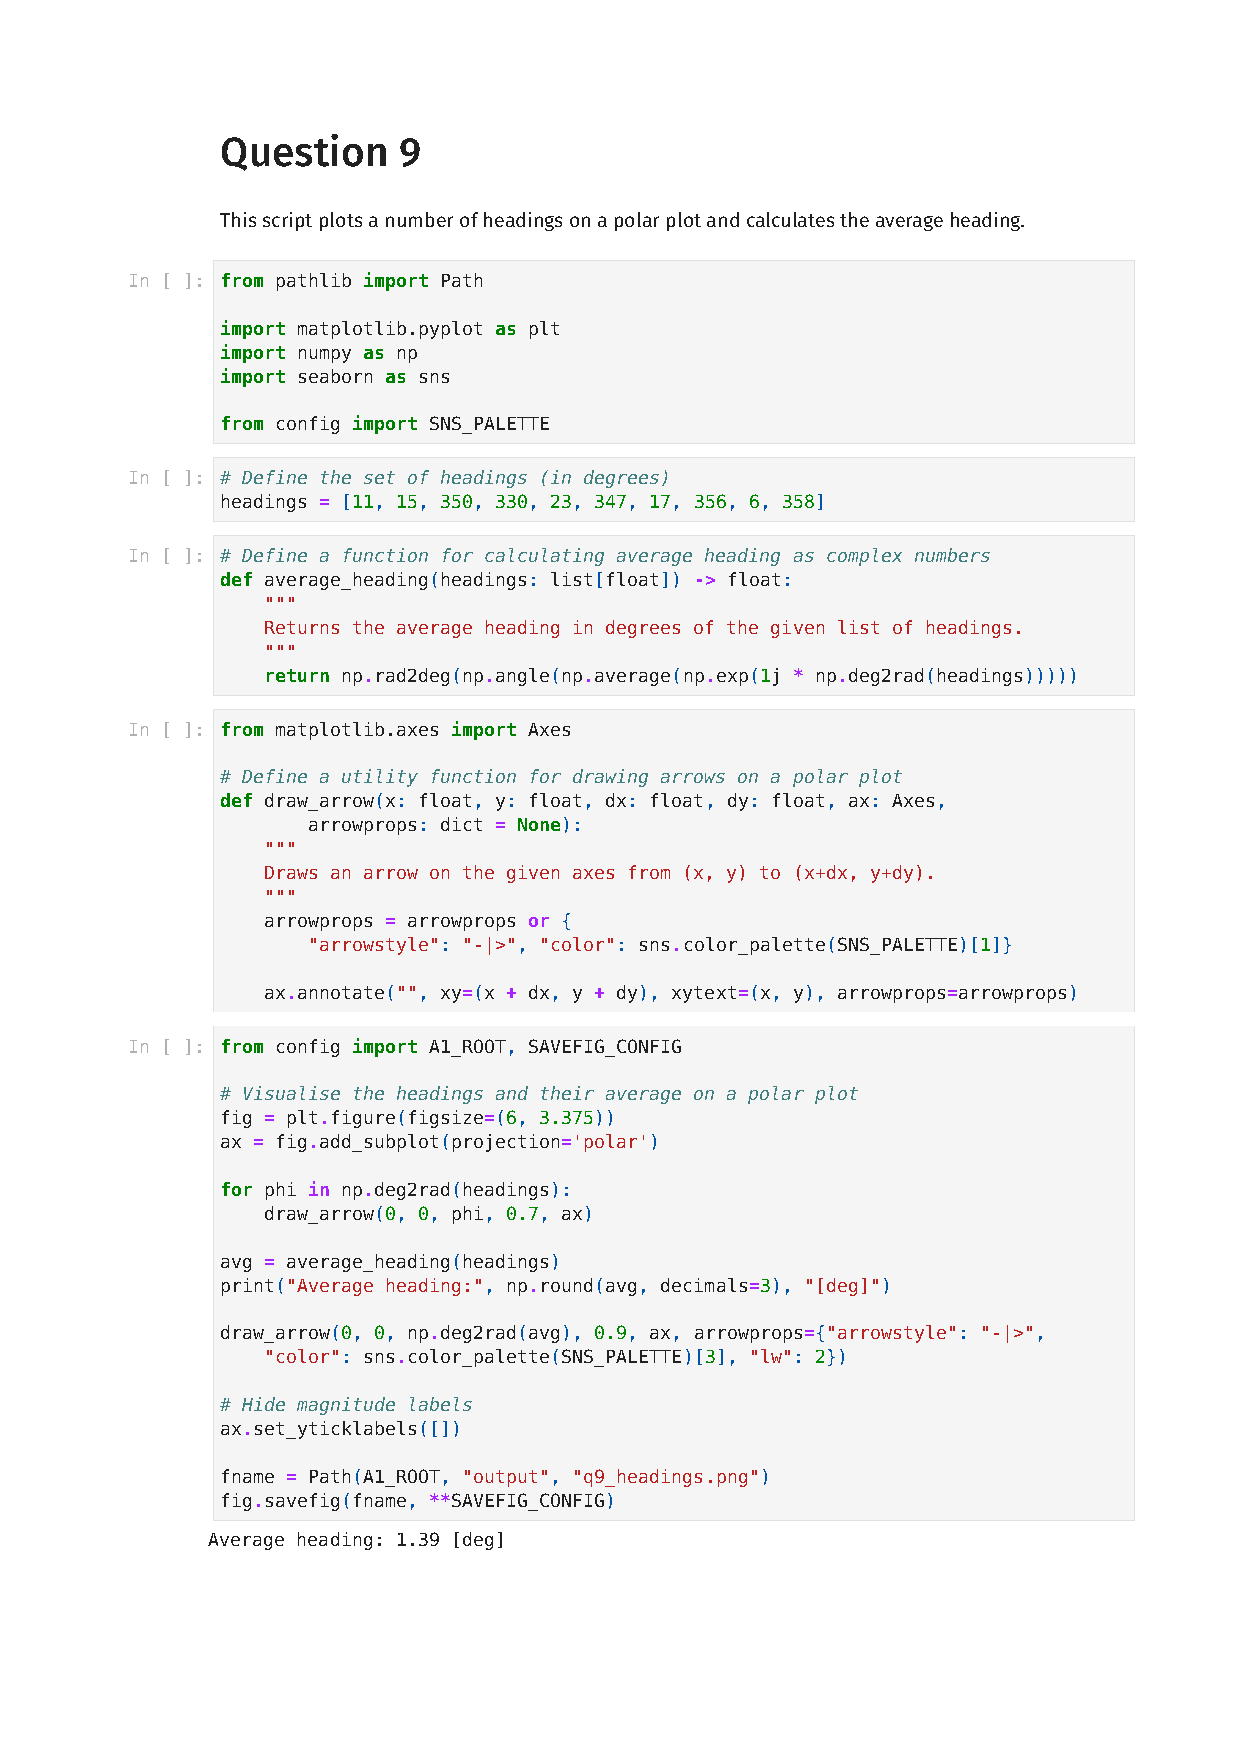
\includepdf[pages=-]{pdfpages/q9_headings.pdf}

\end{document}
